\documentclass[a4paper,11pt]{book}
%\documentclass[a4paper,twoside,11pt,titlepage]{book}
\usepackage{listings}
\usepackage[utf8]{inputenc}
\usepackage[USenglish,spanish,es-tabla]{babel}
\usepackage{multirow}
\usepackage{float}	
\usepackage{subfigure}
\usepackage{lscape}
\usepackage{amssymb, amsmath, amsbsy}

% \usepackage[style=list, number=none]{glossary} %
%\usepackage{titlesec}
%\usepackage{pailatino}

\decimalpoint
\usepackage{dcolumn}
\newcolumntype{.}{D{.}{\esperiod}{-1}}
\makeatletter
\addto\shorthandsspanish{\let\esperiod\es@period@code}\makeatother


%\usepackage[chapter]{algorithm}
\RequirePackage{verbatim}
%\RequirePackage[Glenn]{fncychap}
\usepackage{fancyhdr}
\usepackage{graphicx}
\usepackage{afterpage}
\usepackage{longtable}

\usepackage[pdfborder={000}]{hyperref} %referencia

% ********************************************************************
% Re-usable information
% ********************************************************************
\newcommand{\myTitle}{MEDA-Toolbox: Interfaz Gráfica en Matlab para la detección de anomalías en red\xspace}
\newcommand{\myDegree}{Grado en Ingeniería informática\xspace}
\newcommand{\myName}{Pablo Sánchez Robles (alumno)\xspace}
\newcommand{\myProf}{José Camacho Páez (tutor)\xspace}
\newcommand{\myFaculty}{Escuela Técnica Superior de Ingenierías Informática y de Telecomunicación\xspace}
\newcommand{\myFacultyShort}{E.T.S. de Ingenierías Informática y de Telecomunicación\xspace}
\newcommand{\myDepartment}{Departamento de Teoría de la Señal, Telemática y Comunicaciones\xspace}
\newcommand{\myUni}{\protect{Universidad de Granada}\xspace}
\newcommand{\myLocation}{Granada\xspace}
\newcommand{\myTime}{\today\xspace}
\newcommand{\myVersion}{Version 0.1\xspace}


\hypersetup{
pdfauthor = {\myName (pablosanchez@correo.ugr.es)},
pdftitle = {\myTitle},
pdfsubject = {Trabajo de Fin de Grado},
pdfkeywords = {Análisis exploratorio de datos, MEDA-Toolbox, Detección de ataques en red, Big Data},
pdfcreator = {LaTeX},
pdfproducer = {pdflatex}
}

%\hyphenation{}


%\usepackage{doxygen/doxygen}
%\usepackage{pdfpages}
\usepackage{url}
\usepackage{colortbl,longtable}
\usepackage[stable]{footmisc}
%\usepackage{index}

%\makeindex
%\usepackage[style=long, cols=2,border=plain,toc=true,number=none]{glossary}
% \makeglossary

% Definición de comandos que me son tiles:
%\renewcommand{\indexname}{Índice alfabético}
%\renewcommand{\glossaryname}{Glosario}

\pagestyle{fancy}
\fancyhf{}
\fancyhead[LO]{\leftmark}
\fancyhead[RE]{\rightmark}
\fancyhead[RO,LE]{\textbf{\thepage}}
\renewcommand{\chaptermark}[1]{\markboth{\textbf{#1}}{}}
\renewcommand{\sectionmark}[1]{\markright{\textbf{\thesection. #1}}}

\setlength{\headheight}{1.5\headheight}

\newcommand{\HRule}{\rule{\linewidth}{0.5mm}}
%Definimos los tipos teorema, ejemplo y definición podremos usar estos tipos
%simplemente poniendo \begin{teorema} \end{teorema} ...
\newtheorem{teorema}{Teorema}[chapter]
\newtheorem{ejemplo}{Ejemplo}[chapter]
\newtheorem{definicion}{Definición}[chapter]

\definecolor{gray97}{gray}{.97}
\definecolor{gray75}{gray}{.75}
\definecolor{gray45}{gray}{.45}
\definecolor{gray30}{gray}{.94}

\lstset{ frame=Ltb,
     framerule=0.5pt,
     aboveskip=0.5cm,
     framextopmargin=3pt,
     framexbottommargin=3pt,
     framexleftmargin=0.1cm,
     framesep=0pt,
     rulesep=.4pt,
     backgroundcolor=\color{gray97},
     rulesepcolor=\color{black},
     %
     stringstyle=\ttfamily,
     showstringspaces = false,
     basicstyle=\scriptsize\ttfamily,
     commentstyle=\color{gray45},
     keywordstyle=\bfseries,
     %
     numbers=left,
     numbersep=6pt,
     numberstyle=\tiny,
     numberfirstline = false,
     breaklines=true,
   }
 
% minimizar fragmentado de listados
\lstnewenvironment{listing}[1][]
   {\lstset{#1}\pagebreak[0]}{\pagebreak[0]}


\lstdefinestyle{Consola}
   {basicstyle=\scriptsize\bf\ttfamily,
    backgroundcolor=\color{gray30},
    frame=single,
    numbers=none
   }

\newcommand{\bigrule}{\titlerule[0.5mm]}


%Para conseguir que en las páginas en blanco no ponga cabecerass
\makeatletter
\def\clearpage{%
  \ifvmode
    \ifnum \@dbltopnum =\m@ne
      \ifdim \pagetotal <\topskip
        \hbox{}
      \fi
    \fi
  \fi
  \newpage
  \thispagestyle{empty}
  \write\m@ne{}
  \vbox{}
  \penalty -\@Mi
}
\makeatother

\usepackage{pdfpages}
\begin{document}
\begin{titlepage}
 
 
\newlength{\centeroffset}
\setlength{\centeroffset}{-0.5\oddsidemargin}
\addtolength{\centeroffset}{0.5\evensidemargin}
\thispagestyle{empty}

\noindent\hspace*{\centeroffset}\begin{minipage}{\textwidth}

\centering

\includegraphics[width=0.9\textwidth]{imagenes/logo_ugr.jpg}\\[1.4cm]

\textsc{ \Large TRABAJO FIN DE GRADO\\[0.2cm]}
\textsc{ INGENIERÍA EN INFORMÁTICA}\\[1cm]
% Upper part of the page
% 
% Title
{\Huge\bfseries MEDA-Toolbox: Interfaz Gráfica en Matlab para la detección de anomalías en red}
\noindent\rule[-1ex]{\textwidth}{3pt}\\[3.5ex]
\end{minipage}

\vspace{2.5cm}
\noindent\hspace*{\centeroffset}\begin{minipage}{\textwidth}
\centering

\textbf{Autor}\\ {Pablo Sánchez Robles (alumno)}\\[2.5ex]
\textbf{Directores}\\
{José Camacho Páez (tutor)}\\[2cm]

\includegraphics[width=0.3\textwidth]{imagenes/etsiit_logo.png}\\[0.1cm]
\textsc{Escuela Técnica Superior de Ingenierías Informática y de Telecomunicación}\\
\textsc{---}\\
Granada, mes de 2015
\end{minipage}
%\addtolength{\textwidth}{\centeroffset}
%\vspace{\stretch{2}}
\end{titlepage}



\chapter*{}
%\thispagestyle{empty}
%\cleardoublepage

%\thispagestyle{empty}

%\begin{titlepage}
 
 
\setlength{\centeroffset}{-0.5\oddsidemargin}
\addtolength{\centeroffset}{0.5\evensidemargin}
\thispagestyle{empty}

\noindent\hspace*{\centeroffset}\begin{minipage}{\textwidth}

\centering
%
\includegraphics[width=0.9\textwidth]{imagenes/logo_ugr.jpg}\\[1.4cm]

%\textsc{ \Large PROYECTO FIN DE CARRERA\\[0.2cm]}
%\textsc{ INGENIERÍA EN INFORMÁTICA}\\[1cm]
% Upper part of the page
% 

 \vspace{3.3cm}

%si el proyecto tiene logo poner aquí

\includegraphics{imagenes/logo.png} 
 \vspace{0.5cm}

% Title

{\Huge\bfseries Título del proyecto\\
}
\noindent\rule[-1ex]{\textwidth}{3pt}\\[3.5ex]
{\large\bfseries Subtítulo del proyecto.\\[4cm]}
\end{minipage}

\vspace{2.5cm}
\noindent\hspace*{\centeroffset}\begin{minipage}{\textwidth}
\centering

\textbf{Autor}\\ {Nombre Apellido1 Apellido2 (alumno)}\\[2.5ex]
\textbf{Directores}\\
{Nombre Apellido1 Apellido2 (tutor1)\\
Nombre Apellido1 Apellido2 (tutor2)}\\[2cm]
%
\includegraphics[width=0.15\textwidth]{imagenes/tstc.png}\\[0.1cm]
%\textsc{Departamento de Teoría de la Señal, Telemática y Comunicaciones}\\
%\textsc{---}\\
%Granada, mes de 201
\end{minipage}
%\addtolength{\textwidth}{\centeroffset}
\vspace{\stretch{2}}

 
\end{titlepage}






%\cleardoublepage
\thispagestyle{empty}

\begin{center}
{\large\bfseries  MEDA-Toolbox: Interfaz Gráfica en Matlab para la detección de anomalías en red}\\
\end{center}
\begin{center}
Pablo Sánchez Robles  (alumno)\\
\end{center}

%\vspace{0.7cm}
\noindent{\textbf{Palabras clave}: Análisis exploratorio de datos, MEDA-Tooblox, Big Data, detección de anomalías en red, datos de seguridad en red, AED, GUIDE}

\vspace{0.7cm}
\noindent{\textbf{Resumen}}\\

En el presente documento se pretende desarrollar una interfaz gráfica para análisis de BIG DATA haciendo uso de la Toolbox MEDA, y orientar dicha interfaz a la detección de anomalías en redes de computadores con un amplio número de conexiones y usuarios finales.
\bigskip

Se comenzará por estudiar las metodologías que se utilizarán para la disminución del tamaño del problema y para la identificación de los elementos notables, ya sea porque generan las anomalías en el funcionamiento correcto del sistema o porque no se tienen encuadrados dentro de los parámetros normales. Se dará una introducción sobre el concepto de BIG DATA y los grandes conjuntos de datos.
\bigskip

También se hará un breve resumen de la historia de la seguridad informática así como de los elementos a tener en cuenta dentro de los sistemas para a detección de las fallas en la seguridad.
\bigskip

Se hará la ingeniería del software pertinente para el desarrollo de la interfaz y se finalizará con un caso de estudio que pondrá a prueba lo desarrollado a lo largo de todo el trabajo.

\cleardoublepage


\thispagestyle{empty}


\begin{center}
{\large\bfseries MEDA-Toolbox: Graphic user interface in Matlab for network anomaly detection}\\
\end{center}
\begin{center}
Pablo Sánchez Robles (student)\\
\end{center}

%\vspace{0.7cm}
\noindent{\textbf{Keywords}: Exploratory Data Analisys, MEDA-Toolbox, Big Data, Network Anomaly Detection, Security data network , EDA, GUIDE}\\

\vspace{0.7cm}
\noindent{\textbf{Abstract}}\\

Herein it is intended to develop a graphical interface for BIG DATA analysis by using the MEDA toolbox and head such an  interface for the detection of anomalies in computer networks with a large number of connections and end users.
\bigskip

We will start studying the methodologies to be used for reducing the size of the problem and for identifying the significant items,either because they generate anomalies in the proper functioning of the system or because they are not framed within  normal parameters . An  introduction to the concept of BIG DATA and large data sets will be given.
\bigskip

A brief summary of the history of the computer security as well as the elements to be considered within the systems for the detection of security breaches will also be done.
\bigskip

Engineering to the development of   relevant interface software will be made and  by ending up with a case study that  will test everything  that has been  developoled throughout the work
\bigskip

\chapter*{}
\thispagestyle{empty}

\noindent\rule[-1ex]{\textwidth}{2pt}\\[4.5ex]

Yo, \textbf{Pablo Sánchez Robles}, alumno de la titulación Ingenría Informática de la \textbf{Escuela Técnica Superior
de Ingenierías Informática y de Telecomunicación de la Universidad de Granada}, con DNI 75159703-G , autorizo la
ubicación de la siguiente copia de mi Trabajo Fin de Grado en la biblioteca del centro para que pueda ser
consultada por las personas que lo deseen.

\vspace{6cm}

\noindent Fdo: Pablo Sánchez Robles

\vspace{2cm}

\begin{flushright}
Granada a X de mes de 2015 .
\end{flushright}


\chapter*{}
\thispagestyle{empty}

\noindent\rule[-1ex]{\textwidth}{2pt}\\[4.5ex]

D. \textbf{José Camacho Páez}, Profesor del Área de Ingeniería Telemática del Departamento Teoría de la Señal, Telemática y Comunicaciones de la Universidad de Granada.

\vspace{0.5cm}

\vspace{0.5cm}

\textbf{Informan:}

\vspace{0.5cm}

Que el presente trabajo, titulado \textit{\textbf{MEDA-Toolbox: Interfaz Gráfica en Matlab para la detección de anomalías en red}},
ha sido realizado bajo su supervisión por \textbf{Pablo Sánchez Robles}, y autorizamos la defensa de dicho trabajo ante el tribunal
que corresponda.

\vspace{0.5cm}

Y para que conste, expiden y firman el presente informe en Granada a X de mes de 2015 .

\vspace{1cm}

\textbf{Los directores:}

\vspace{5cm}

\noindent \textbf{José Camacho Páez}

\chapter*{Agradecimientos}
\thispagestyle{empty}

       \vspace{1cm}


	A mis padres, mi hermana y mi cuñado por aguantarme día a día como lo han hecho y por estar siempre ahí para todo lo que me ha hecho falta.
	\bigskip
	
	A mis amigos por ser la vía de escape en los momentos difíciles y no fallarme en ningún momento.
	\bigskip
	
	A mis compañeros de la ETSIIT por darlo todo cuando se les necesita y por hacer del trabajo en equipo un sistema de vida.
	\bigskip
	
	A mis abuelos por inculcarme el valor por el estudio desde que tengo uso de razón.
	\bigskip
	
	Especialmente a todos los que ya no están porque la marca que han dejado jamás se perderá.
 


\frontmatter
\tableofcontents
\listoffigures
\listoftables

\mainmatter
%\setlength{\parskip}{5pt}

\chapter{Introducción}

En el presente trabajo se va a exponer el desarrollo de una interfaz gráfica de usuario para una herramienta de análisis de datos y tratamiento de Big Data para la detección de anomalías en tráfico de red.
\bigskip

\section{Contexto histórico de la seguridad}  

\cite{CHS} \cite{ISS} Históricamente el primer ataque contra la seguridad informática se produjo en 1972 por Robert Thomas Morris quien creó el primer virus reconocido como tal cuyo nombre era \textbf{Creeper}, un software bastante sencillo que sólo mostraba regularmente un mensaje por pantalla \textbf{I am a creep, catch me if you can} y se movía a otros sistemas a los que estuviera conectado, en ese momento no se pretendía llegar a colapsar sistemas o capturar información confidencial. En contramedida a este “virus” se creó \textbf{Reaper} que técnicamente era otro virus que también se movía entre máquinas pero con la finalidad de eliminar al anterior.
\bigskip

\cite{PVI}El primer virus con mecanismos de propagación reales llegó en 1983 de la mano de Fred Cohen que desarrolló como experimento un software que modificaba otros programas para insertar su código en ellos y que éstos a su vez hicieran lo mismo construyendo así el primer gusano de la historia.
\bigskip

Tras esto los virus fueron evolucionando hasta llegar el primer polimórfico  en 1990 llamado \textbf{“Dark avenger mutation engine”} que cambiaba de forma en cada infección para dificultar su identificación.
\bigskip

En 1989 se creó \textbf{“Stoned”} un virus que infectaba el sector de arranque del disco duro contando el número de reinicios y mostrando un mensaje, no tuvo mayor repercusión hasta que en 1992 se crea \textbf{“Michelangelo”} una variante de él que infectaba los 100 primeros sectores del disco inutilizándolo, este fue el primero virus que inició el pánico mediático entorno a la informática.
\bigskip

A partir de este momento se fueron creando antivirus más completos, puesto que hasta finales de los 80 sólo se creaban programas como respuesta a los virus concretos pero no globales. No sólo buscaban programas en particular si no que escaneaban en busca de comportamientos anómalos o inapropiados.
\bigskip

\cite{CIH} En 1998 apareció \textbf{“CIH”}, el virus  más destructivo hasta el momento infectando más de 60 millones de máquinas e inutilizándolas puesto que sobrescribía la BIOS impidiendo el arranque de las mismas, produjo grandes daños económicos.
\bigskip

Hasta este punto los ataques se basaban en virus  que infectaban, se replicaban y cambiaban de forma siguiendo unos patrones y que básicamente interrumpían el funcionamiento normal de las máquinas, pero a partir del año 2000 comenzaron a implementarse nuevas técnicas de ataque. Técnicas utilizadas para acceder a los sistemas y tomar control de ellos como pueden ser los \textbf{ataques de autenticación}, bloquear servicios que ofrezcan con \textbf{denegación de servicio (DoS)}, robar información de los usuarios de una red con \textbf{ataques de monitorización}, aprovechando la “credulidad” o falta de conocimiento de los usuarios para robarles información con \textbf{ingeniería social}  o \textbf{ataques de modificación}  para cambiar transmisiones de datos, configuraciones de usuario o borrar las huellas de un ataque.
\bigskip

En la actualidad vivimos en una sociedad interconectada por multitud de dispositivos que comparten información de naturaleza muy diferente entre las que se encuentran datos sensibles de los usuarios, dichos datos circulan por la red dependiendo en muchos casos de la seguridad de la misma (aunque pueden venir previamente cifrados o protegidos).
\bigskip

Actualmente las redes son atacadas constantemente con el fin de obtener beneficio económico, suplantar identidades, captación de información confidencial, etc. 

\bigskip 

\section{Motivación}

El presente documento viene motivado por la necesidad que existe de detectar ataques a la seguridad en tiempo real y poder actuar en consecuencia evitando males mayores. Puesto que el problema a tratar va aumentando constantemente debido al crecimiento de las redes de dispositivos (sobre todo móviles) se deben crear mecanismos que permitan llevar a cabo esta tarea de forma automatizada y relativamente sencilla.
\bigskip

Por ello la motivación de este trabajo es el desarrollo de una herramienta para la detección de fallas en la seguridad así como de los elementos de la red que producen estos problemas incluyendo a los usuarios que manejan dichos dispositivos. Para poder llevar a cabo esto se necesitan técnicas que permitan identificar dentro de un conjunto enorme de datos cuál o cuáles son anomalías y analizarlas para encontrar las causas.

\section{Objetivos}

Se pretende con este proyecto llevar a cabo una interfaz gráfica de usuario que permita simplificar el análisis y diagnóstico de los ataques en un entorno de grandes conjuntos de datos como puede ser una red móvil, una red corporativa, etc. 
\bigskip

Para llevar a cabo todo esto se va a utilizar como base del desarrollo la “MEDA-Toolbox” desarrollada por el tutor del presente proyecto José Camacho Páez, en la que también han contribuido Elena Jiménez Mañas, Alejandro Pérez Villegas y Rafael Rodríguez Gómez.
\bigskip

A grandes rasgos los objetivos a cumplir son:

\begin{itemize}
	\item \textbf{OBJ-1:}Estudiar y realizar una introducción teórica de las técnicas estadísticas que utiliza el Análisis Exploratorio de Datos y del análisis de grandes conjuntos de datos.
	
	\item \textbf{OBJ-2:}Tratar el tema de la extracción de datos en red para el estudio de la seguridad.
	
	\item \textbf{OBJ-3:}Análizar, diseñas y desarrollar una interfaz gráfica de manejo sencillo para la utilización de la “MEDA-Toolbox”.
	
	\item \textbf{OBJ-4:}Demostrar la funcionalidad del software mediante un ejemplo con datos reales de una red corporativa.
	
\end{itemize}
\bigskip

En los siguientes capítulos se tratará en detalle las técnicas estadísticas a utilizar (tema 2), las herramientas para el análisis de Big Data (tema 3), Los datos de seguridad en red necesarios para llevar a cabo el estudio (tema 4), la planificación y estimación de costes (tema 5), una descripción de cómo  utilizar la GUIDE de Matlab (tema 6), el proceso de análisis, diseño y desarrollo de la interfaz (temas 7, 8 y 9), un ejemplo de uso del sistema desarrollado con datos reales (tema 10) y por último las conclusiones y el trabajo futuro (tema 11).
%
\chapter{Análisis Exploratorio de Datos} \cite{LSBM} \cite{PHPDAT}

El análisis exploratorio de datos o EDA de sus siglas en inglés “Exploratory Data Analysis” es un procedimiento estadístico que sirve de herramienta para el tratamiento de datos con el fin de encontrar relaciones en los datos obtenidos en diferentes tipos de estudios. 

\bigskip

De metodología relativamente sencilla y sistemática puede organizar los datos para encontrar conjuntos con relaciones fuertes entre sus observaciones (clusters), observaciones que se encuentran fuera de esas relaciones (outliers) y mediante el estudio de estas últimas comprobar si están fuera de esos rangos por errores en las mediciones o por ser casos especiales de estudio.

\bigskip

EDA trata de hacer un análisis cualitativo de los datos para poder extraer información relevante de los mismos. En primer lugar se organizan los datos para el estudio mediante una estandarización de las variables de manera que podamos aplicar las técnicas estadísticas para conseguir la media, varianza, covarianza y demás modelos multivariantes del conjunto a estudiar. A continuación se realiza una visualización de las relaciones existentes. Y por último estudiar los patrones “especiales” como los outliers para ver porqué lo son y si nos son de utilidad en la investigación.

\bigskip

En el siguiente apartado se expondrán las técnicas de proyección de EDA que se van a utilizar en este trabajo.

\bigskip

\section{Técnicas de proyección}
Dentro de todas las posibles técnicas a utilizar para el análisis exploratorio de datos, en este proyecto se van a desarrollar dos principalmente y luego se comentarán algunas de las herramientas mediante las cuales se aplicarán dichas técnicas.
\bigskip 

Las técnicas a utilizar son el análisis de componentes principales o \textbf{PCA} “Principal Component Analysis” y mínimos cuadrados parciales o \textbf{PLS} “Parcial Least Squares”. Por otra parte también existen muchas técnicas gráficas para representar de manera visual los conjuntos de datos como son los gráficos “Score Plots”, “Loading Plots”, MEDA, oMEDA, etc.
\bigskip

Tanto PCA como PLS tratan el mismo problema de la colinealidad de los datos pero en casos diferentes.
\bigskip

Mientras que PCA es mas útil en problemas no supervisados PLS se emplea para los supervisados.
\bigskip
 
Los problemas supervisados son en los que se dispone de información de clases, estando los datos categorizados y haciendo posible el establecimiento de un modelo que ayude a la obtención de resultados en futuros análisis.
\bigskip

Los problemas no supervisados son para los que no hay un propósito específico, no se han seleccionado un conjunto de muestras, ni de variables con las que relacionarlas. Se trabaja sobre un conjunto de datos obtenido sin supervisión y sólo se puede llevar a cabo un análisis para encontrar tendencias o patrones en los mismos, para clasificarlos.
\bigskip

Ambos métodos (PCA y PLS)se basan en la utilización de variables latentes o LVs. Estas variables en PCA se llaman componentes principales o PC y se infieren a partir de la varianza de los datos. En el caso de PLS las se obtienen de la covarianza. 
\bigskip

La reducción del tamaño es esencial cuando tratamos con “Big Data”, donde  cualquier disminución del tamaño del problema agiliza el trabajo, por ello estas técnicas son de gran importancia para el propósito de este proyecto.
\bigskip


\section{Análisis de componentes principales PCA} \cite{EKE} \cite{JMMD}

En este tipo de análisis se utilizan los PCs como se ha comentado en el apartado anterior, los cuales nos ayudan a reducir el tamaño del problema puesto que al inferirlos se eliminan los datos redundantes o repetidos. 
\bigskip

Estas nuevas variables obtenidas son combinaciones lineales de las variables del conjunto de datos inicial. Lo que se pretende con esto es que de un conjunto inicial M  obtener un conjunto A siendo $ A \leq M $. En el caso que M y A fueran iguales el proceso de obtención de las componentes principales no ha reducido el tamaño del problema, lo cual quiere decir que no existe redundancia en los datos ni repetición de los mismos.
\bigskip

En PCA tenemos una matriz, llamémosla X, de tamaño NxM donde las columnas son las variables del estudio y las filas o tuplas son muestras de la población a estudiar u observaciones. La forma de dicha matriz sería X = estructura + residuo, siendo más concretos 

%
\begin{equation}
X= T_A*P_A’ + E_A
\end{equation} 

Donde $T_A$ es la matriz de puntuaciones, que almacena las proyecciones de las observaciones en los PCs, $P_A$ es la matriz de cargas con los autovectores del producto cruzado $X'*X$, $E_A$ es la matriz de residuos, y A es el número de PCs. 
\bigskip

\begin{figure}[H]
\centering
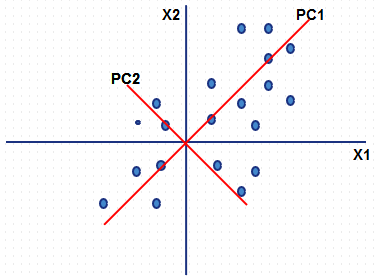
\includegraphics[width=0.9\textwidth]{imagenes/figuras/2_1.png}
\caption{Descripción gráfica de componente principal.}
\end{figure}

Los componentes principales se pueden calcular como combinaciones lineales de las variables originales minizando la suma de cuadrados de las distancias de cada punto al subespacio, maximizando la variabilidad o con regresiones alternas.
\bigskip

Previamente al cálculo de las componentes principales se hace el “centrado de datos” mediante el cual, calculada la media de los valores, se trasladan los ejes de coordenadas a ese punto intermedio, esto se hace restando a cada punto el valor de la media del conjunto, quedando el valor medio en el origen. El número de ejes ortogonales entre sí dependerá del número de componentes principales que se calculen.

\bigskip

En la figura 2.1 se puede ver gráficamente esto, aunque en este caso la dimensión no varía se aprecia como se han representado todo los puntos mediante PC1 y PC2.

\bigskip

Una vez realizada la selección de las variables latentes se pasaría a estudiar las relaciones entre observaciones mediante gráficos como los que se comentarán en los siguientes apartados.
\bigskip


\section{Mínimos cuadrados parciales PLS}
Esta técnica de proyección de datos se da en entornos supervisados, es decir, cuando se dispone de una o varias variables respuesta que guían la exploración. A diferencia del caso anterior las variables latentes que este modelo utiliza se obtienen de la covarianza entre X e Y. El modelo tiene como estructura:

\begin{equation}
X= T_A*P_A^T+E_A
\end{equation}

\begin{equation}
Y= T_A*Q_A^T+F_A
\end{equation}

Donde \textbf{$P_A$}  y \textbf{$Q_A$} son las matrices de carga de tamaño \textbf{A} (número de variables latentes), \textbf{$T_A$} son las matrices de puntuaciones y \textbf{$E_A$} y \textbf{$F_A$} son las de residuos.
\bigskip
También se puede obtener la matriz Y a partir de la X mediante la siguiente función:
\begin{equation}
Y=X*B_A+F_A
\end{equation}


Donde la matriz \textbf{$B_A$} añade los coeficientes de regresión.

\bigskip
Dentro de este método existe una variante  llamada “Mínimos cuadrados parciales – Análisis discriminante” en el que la matriz Y se genera artificialmente con variables “dummy”, una por cada clase del conjunto de datos original. La pertenencia de una variable a una clase se identifica dándole valor uno a la clase que pertenezca y -1 al resto.

\bigskip

\section{Análisis Exploratorio de Datos Multivariante}
\subsection{MEDA}
Dentro de las herramientas del análisis exploratorio de datos se encuentra \textbf{MEDA}, que es una técnica basada en la comparación de variables de forma múltiple. No se basa en el análisis individual de cada una de las variables del conjunto por separado si no en una visión global de las mismas estudiando sus relaciones y cómo de correladas se encuentran entre sí.
\bigskip

En el caso que ocupa este proyecto estudiaremos las formas de visualizar dichas relaciones mediante distintos tipos de gráficos que nos mostraran a simple vista los vínculos, si existen, entre variables
\bigskip

La matriz MEDA que se genera es de tamaño \textbf{MxM}, siendo \textbf{M} el número de variables. En cada una de las celdas de \textbf{M} se almacenará un valor entre -1 y 1 que corresponde a la relación que existe entre la variable i y la j, creándose así una estructura con todas las relaciones posibles. Esta relación se calcula cómo: 
\begin{equation}
q^2_{A,(m,l)}=1-\frac{\parallel \widehat{e}_{A,(l)}\parallel ^2}{\parallel x_{(l)} \parallel ^2} ,\forall l \neq m
\end{equation}


Donde \textbf{$q_{A,(m,l)}$} es cada uno de los valores de la matriz MEDA, \textbf{$\widehat{e}_{A,(l)}$} corresponde a cada uno de los errores en la estimación de la variable \textbf{l} y \textbf{$x_{(l)}$}  es el valor de la variable en análisis. De esta ecuación podemos entender el funcionamiento de MEDA de forma rápida ya que lo que aquí se expresa es que cada uno de los valores de la matriz MEDA será más próximo a cero cuanto mayor sea el error y más próximo a 1 o -1 cuanto mejor sea la estimación.
\bigskip

Utilizando MEDA junto con los modelos de proyección anteriores (PLS y PCA) podremos comprender mejor las relaciones entre variables, ya que mientras que las técnicas de proyección vistas reducen el tamaño del problema y eliminan la colinealidad de los datos, MEDA se encarga de la correlación entre variables.
\bigskip

Con los gráficos MEDA podemos observar mediante un “código de colores” lo relacionadas que están las variables entre sí. Como los valores de la matriz MEDA van desde el -1 hasta el 1 los colores van desde el azul que representa al -1 al rojo que representa al 1, el cero es representado por el blanco y cada valor entre dichos rangos tendrá un color degradado dentro de los mismos. Si el valor se acerca a cero por debajo, es decir -0.1 por ejemplo el color que se verá en el gráfico es un azul muy claro, mientras que si es por arriba, como el 0.1 se verá de un rojo difuminado casi blanco.
\bigskip

\begin{figure}[H]
\centering
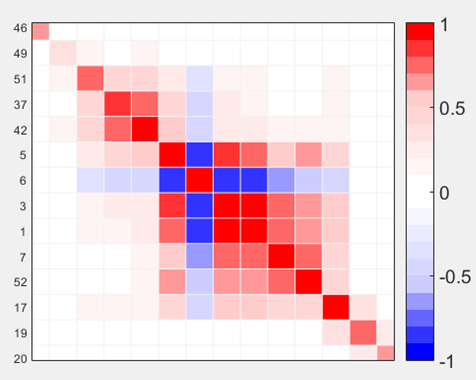
\includegraphics[width=0.9\textwidth]{imagenes/figuras/2_3.png}
\caption{Ejemplo de gráfico MEDA.}
\end{figure}

La figura 2.2 muestra un ejemplo de gráfico MEDA,  ampliado para que sólo se muestre una parte del mismo, de esta forma se pueden apreciar los distintos degradados de color escalados por los colores de la derecha de la imagen. Se puede ver como la variable 5 y la 6 tienen una fuerte relación pero inversa, mientras que la 5 con la 3 tienen una fuerte relación directa.

\bigskip

\subsection{oMEDA}

Este método derivado del anterior se encarga de relacionar variables con observaciones para ver cuáles de ellas (variables) están más relacionadas con patrones descritos en las observaciones.
\bigskip

Este método aplica MEDA sobre los datos originales con una variable que represente las observaciones de interés, incluyéndola en el conjunto de variables mediante un vector columna que da valores a cada observación dividiendo el conjunto en grupos de observaciones a comparar.
\bigskip

Éste método da valores de 1, 0 y -1 en dicho vector de observaciones siendo 1 las observaciones a estudiar, -1 a los datos con los que se quiere comparar dichas observaciones y 0 a todas las que no se quieren estudiar, ignorando por tanto oMEDA todas las variables que tengan dicho 0.
\bigskip

\begin{figure}[H]
\centering
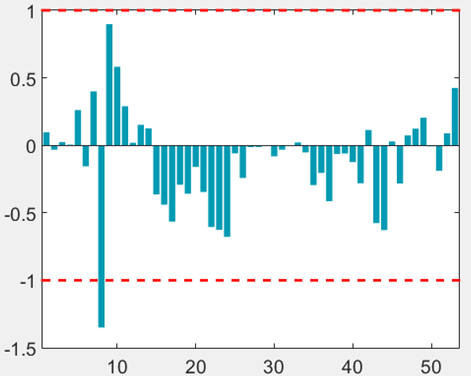
\includegraphics[width=0.9\textwidth]{imagenes/figuras/2_4.png}
\caption{Ejemplo de oMEDA.}
\end{figure}

\bigskip

En la figura 2.3 se tiene un ejemplo de oMEDA, en el que se puede apreciar como dentro del conjunto de observaciones seleccionado la variable 8 y la 9 son las que mas importancia toman en la relación.

\subsection{Score Plots}

Este tipo de gráficos se utilizan para ver de forma rápida la distribución de las observaciones en el sub-espacio de variables latentes por parejas de las mismas. 
\bigskip

En un eje de coordenadas se sitúa una variable y en el otro otra, elegidas por el analista, y así podemos observar la existencia de clusters, outliers o cualquier tipo de patrón en los datos que nos dé una idea de qué relación existe entre las observaciones. Con este método podemos ver las diferencias existentes entre conjuntos de datos que pueden tener modelos PCA o PLS iguales. Se utiliza para interpretar las relaciones entre las observaciones.

\begin{figure}[H]
\centering
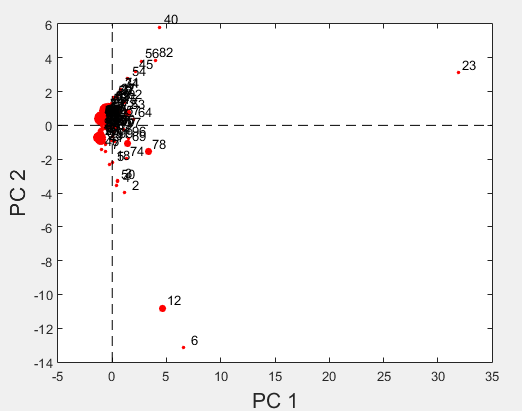
\includegraphics[width=0.9\textwidth]{imagenes/figuras/2_5.png}
\caption{Ejemplo de Score Plot.}
\end{figure}
\bigskip

En la figura 2.4 se pueden observar varios elementos notables, mientras que en el origen de coordenadas se puede ver un cluster, tambien se observan 3 outliers identificados por las etiquetas 23, 12 y 6.

\subsection{Loading Plots}

Similar al anterior los loading plots nos muestran la correlación entre variables. Al igual que el anterior, se seleccionan dos LVs y este gráfico nos muestra lo correladas que están entre sí, viendo si dicha correlación es positiva o negativa. Si dos registros se encuentran muy juntos entre sí podemos decir que su correlación es positiva, mientras que si mantienen una distancia “simétrica” con respecto al origen podemos decir que es negativa. La diferencia con el anterior es que en este caso se utiliza para interpretar las diferencias entre las variables y no entre las observaciones.

\begin{figure}[H]
\centering
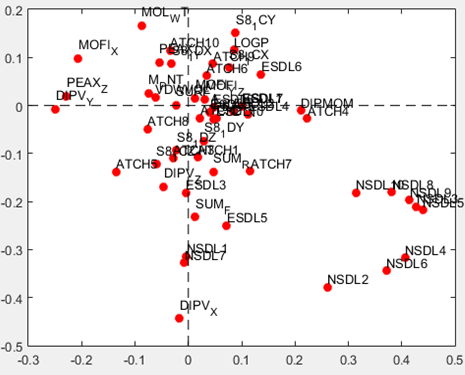
\includegraphics[width=0.9\textwidth]{imagenes/figuras/2_6.png}
\caption{Ejemplo de Loading Plot.}
\end{figure}

En el caso de la figura 2.5 no se pueden apreciar tendencias o patrones en las variables ya que es complicado identificar clusters  u outliers en la visualización.
%
\chapter{Análisis de grandes conjuntos de datos} \cite{BIGD}
En EDA como se ha tratado en el tema anterior se pueden usar distintas herramientas para generar hipótesis que sean de interés utilizando las técnicas que ya se han visto como PCA, PLS, score plots, MEDA, etc.
\bigskip

En concreto los score plots son las técnicas que mejor muestran los patrones que se pueden dar en las observaciones. En este tema se explicará una versión de los mismos orientada a problemas con un número de observaciones ilimitadas o muy grandes. Esta técnica se conoce como “Compressed Score Plots” (CSPs).
\bigskip

También se va a comentar la parte de MEDA-Toolbox que se encarga del tratamiento de Big Data y el resto de los métodos de visualización visto en el capítulo anterior.
\bigskip

Los métodos \textbf{BigData} de la toolbox son capaces de lidiar con conjuntos de datos enormes y con flujos de información constantes a altas velocidades manteniendo las capacidades de visualización vistas anteriormente, en tiempos de análisis similares a los problemas de menor tamaño.
\bigskip

\section{¿Qué es Big Data?}
Las nuevas tecnologías facilitan el flujo de información entre distintos sistemas con capacidades de generación de datos inconmensurables, esta gran cantidad de datos es el llamado Big Data.  En campos como la medicina, la química, la física y en el caso que nos ocupa de las redes de computadores, se llegan a generar tantos datos que hay que inventar nuevas técnicas de análisis de los mismos ya que con las clásicas no se puede abordar su análisis.
\bigskip

La definición de Big Data se puede dar con las llamadas “4 uves”:

\begin{itemize}
	\item \textbf{Variedad:}Los datos son formados por distintas fuentes, con distinta naturaleza y estructura.
	
	\item \textbf{Veracidad:}La búsqueda de información relevante en grandes conjuntos de datos es un trabajo complicado y la relación entre señal-ruido en Big Data es baja, por lo que se necesitan técnicas capaces de encontrar patrones de utilidad en la práctica.
	
	\item \textbf{Volumen:}La cantidad de información que se maneja es muy alta.
	
	\item \textbf{Velocidad:}En problemas de Big Data es normal tener grandes flujos constantes de información necesitando ser analizada, por ello la velocidad con la que se procesan los mismos ha de ser alta para resolver los problemas sin que se acumulen más muestras de lo necesario.
	
\end{itemize}


\section{Limitaciones de los Score Plots para grandes conjuntos de datos}

\begin{figure}[H]
\centering
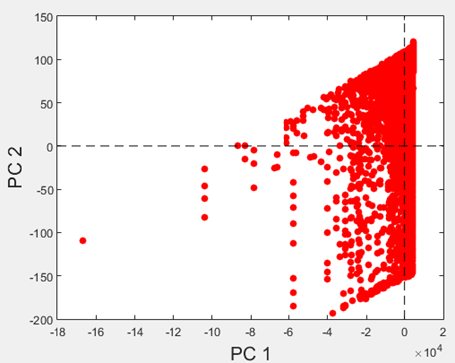
\includegraphics[width=0.9\textwidth]{imagenes/figuras/3_1.png}
\caption{Ejemplo de score plot con BIG DATA.}
\end{figure}

Cuando se utiliza EDA para grandes conjuntos de datos con millones de observaciones que a su vez contienen millones de variables se deben tener en cuenta consideraciones especiales ya que sería imposible dar una representación gráfica comprensible mediante Score plots. Por ello los modelos de proyección de EDA pueden ayudar a reducir el problema pero no lo suficiente para hacer un análisis correcto de lo que sucede.
\bigskip

Como se puede ver en la figura 3.1 en el gráfico es casi imposible establecer patrones o hacerse una idea de las tendencias dentro de un conjunto tan grande de observaciones que emborronan la imagen limitando su utilidad.
\bigskip

Teniendo en cuenta que para el ejemplo de la figura 3.1 se ha utilizado un fichero de datos con 9998 observaciones con 122 variables cada una, y a la hora de analizar Big Data se suelen utilizar varios ficheros de igual o mayor tamaño de forma simultánea, el lector se puede hacer una idea del tamaño del problema a tratar y de como Score plot no es capaz de asimilarlo.

\bigskip
Para solucionar este problema se tiene CSP.

\bigskip

\section{Compressed Score Plots} \cite{CAILS}

El problema de la visualización de Big Data en Score Plots se resuelve mediante técnicas de “clustering”, agrupando observaciones relacionadas mediante gamas de color diferentes para cada cluster, de esta manera se pueden identificar nubes relacionadas a simple vista. 
\bigskip

El criterio que se utiliza para hacer estas agrupaciones es necesario para la creación del cluster, normalmente el más utilizado es el de la distancia. La más popular es la distancia euclídea aunque también se utiliza la distancia de Mahalanobis cuando la diferencia en escala y la correlación de las variables no son despreciables. De forma general la distancia cuadrática se expresa como:
\bigskip

$d_K(x_i-x_j)=\parallel x_i-x_j\parallel_K=((x_i-x_j)^T K^{-1} (x_i-x_j ))^{1/2}$

\bigskip

Donde K es la matriz identidad M-dimensional cuando se utiliza la distancia euclídea y la matriz de covarianza de las variables originales de M en el caso de la distancia Mahalanobis.La inversión de K puede ocasionar problemas al utilizar la distancia de  Mahalanobis. Para evitar dichos problemas se puede restringir dicha inversión a un sub-espacio de proyección como el de PCA o PLS. Dicha inversa de K se calcula:
\bigskip

\begin{itemize}
	\item \textbf{En PCA:} $P*K_{PCA}^{-1}*P^T$
	
	\item \textbf{En PLS:} $P*K_{PLS}^{-1}*P^T$
\end{itemize}

\bigskip

\subsection{Métodos de agrupamiento}
Los métodos de “clustering” o métodos de agrupamiento para Compressed Score Plots, a partir de ahora CSP, no son tarea fácil ya que en el proceso no se pueden destruir datos de interés ni introducir valores inservibles dentro de la distribución de datos. Las técnicas más eficientes para agrupar grandes conjuntos de datos son:
\bigskip

\begin{itemize}
	\item Búsqueda eficiente de vecinos cercanos   
	
	\item Resumen de datos.
	
	\item Computación distribuida.
	
	\item Agrupamiento incremental.
	
	\item Métodos basados en muestreo.
\end{itemize}

De los métodos comentados la Toolbox se basa en el agrupamiento incremental.

\bigskip

\section{Reducción del tamaño del problema}
Para la utilización de las técnicas de visualización vistas en el capítulo anterior en Big Data se necesita reducir el tamaño del problema ya que MEDA y oMEDA tampoco puede manejar problemas con miles de observaciones con cientos de variables cada una. Para esto se calculan lo que en la MEDA-Toolbox se ha llamado la matriz XX, matriz de productos cruzados o matriz de Gram, que es similar salvo una constante a la matriz de covarianzas. Se forma mediante una matriz de datos preprocesados multiplicada por su traspuesta.

\bigskip

\section{Ejemplo de análisis Big Data usando MEDA-Toolbox}

Para este apartado se va a seguir el ejemplo de la Toolbox de “Networkmetrics” orientado a Big Data. Estos datos de ejemplo se pueden encontrar en: \url{https://github.com/josecamachop/MEDA-Toolbox/tree/master/Examples/Networkmetrics}

\bigskip

Se comienza por crear una estructura de datos llamada “Lmodel” que manejará el modelo que caracterizará el análisis, a dicha estructura hay que introducirle los siguientes valores para poder inicializarla:
\bigskip

\begin{itemize}
	\item \textbf{update:}Tiene como valores posibles 1 y 2, que representan: \begin{itemize}
		\item 1 para usar EWMA:Implementa un procesamiento en línea de flujos de datos continuados.
		\item 2 para usar Iterative:Implementa un modo de procesamiento de grandes conjuntos de datos de forma iterativa.
	\end{itemize}
	
	\item \textbf{type:} : Tiene como valores posibles 1 y 2 que representa: \begin{itemize}
		\item 1 para utilizar PCA.
		\item 2 para utilizar PLS.
	\end{itemize}

	\item \textbf{lv:} número de variables latentes. 
	
	\item \textbf{prep:}Escalado o centrado de X. 0 sin escalado, 1 centrado, 2 Auto-escalado.
	
	\item 
	\item \textbf{prepy:}Escalado o centrado de Y. 0 sin escalado, 1 centrado, 2 Auto-escalado.
	
	\item\textbf{nc:}Número de clusters para CSP.
\end{itemize}

\bigskip

Una vez creada la estructura que representara al modelo se pasa a construir el modelo propiamente dicho con los datos de la misma. Según el “update” introducido se creará un modelo “ewma” o un “iterative”. Las funciones de la Toolbox que llevan a cabo esta tarea son “update\_ewma” y “update\_iterative”, ambas dan como objeto de salida un “Lmodel”. 
\bigskip

El siguiente paso es el análisis en sí, que dependiendo del “type” hará un preprocesamiento de los datos PCA o PLS. Las funciones de la Toolbox que se utiliza son “scores\_Lpls”, “meda\_Lpls” y “omeda\_Lpls” para un análisis PLS y análogamente para PCA son “scores\_Lpca”, “meda\_Lpca” y “omeda\_Lpca”. 
\bigskip

En las figuras de la 3.2 en adelante se puede observar cómo las técnicas de análisis de Big Data utilizadas resaltan de entre todos los datos los subconjuntos más relacionados entre sí.
\bigskip

\begin{figure}[H]
\centering
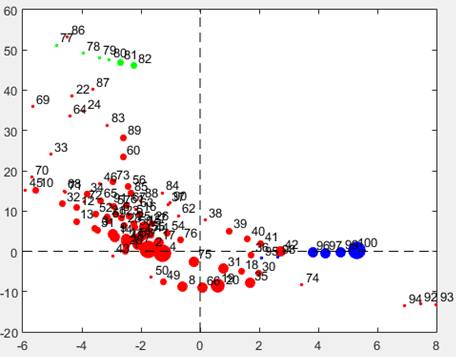
\includegraphics[width=0.8\textwidth]{imagenes/figuras/3_2.png}
\caption{Score plot en iterative y PLS.}
\end{figure}

\begin{figure}[H]
\centering
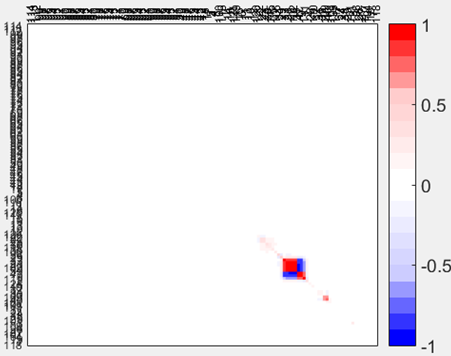
\includegraphics[width=0.8\textwidth]{imagenes/figuras/3_3.png}
\caption{MEDA en iterative y PLS.}
\end{figure}

\begin{figure}[H]
\centering
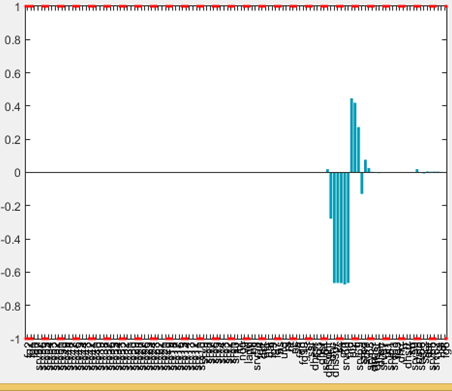
\includegraphics[width=0.8\textwidth]{imagenes/figuras/3_4.png}
\caption{oMEDA en iterative y PLS}
\end{figure}

\bigskip

Cuando se va a analizar conjuntos acotados de datos es más efectivo utilizar el “update” iterative, esto hace un preprocesamiento de los datos de todo el conjunto y después realiza el análisis, como es en el caso de los ejemplos de las figuras 3.2, 3.3 y 3.4. 
\bigskip

\begin{figure}[H]
\centering
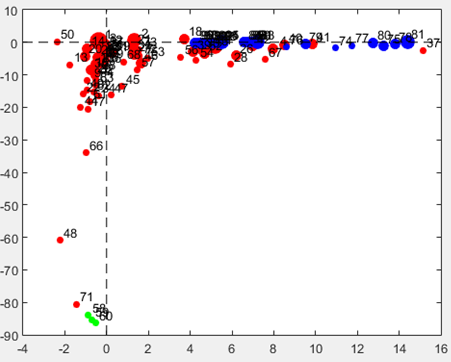
\includegraphics[width=0.8\textwidth]{imagenes/figuras/3_5.png}
\caption{Score plot en EWMA y PCA}
\end{figure}


\begin{figure}[H]
\centering
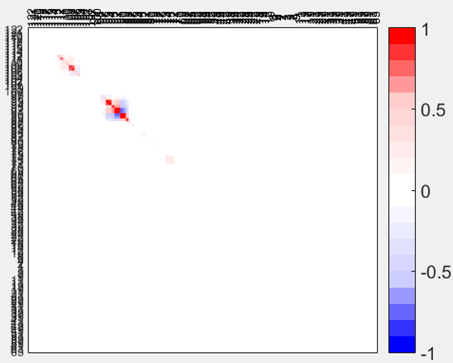
\includegraphics[width=0.8\textwidth]{imagenes/figuras/3_6.png}
\caption{MEDA en EWMA y PCA}
\end{figure}


\begin{figure}[H]
\centering
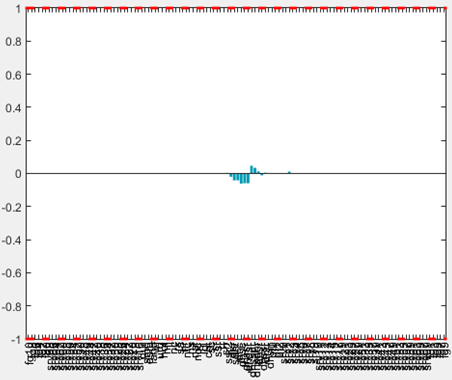
\includegraphics[width=0.8\textwidth]{imagenes/figuras/3_7.png}
\caption{oMEDA en EWMA y PCA}
\end{figure}


La estrategia EWMA utilizada en las figuras 3.5, 3.6, 3.7 se aplica para flujos constantes de datos, como streamings en los que continuamente se está recibiendo nueva información, por ello se usa un factor de olvido llamado en el caso del ejemplo de la Toolbox “lambda”, que va restando importancia a los datos conforme avanza el tiempo, para poder así analizar los nuevos que le van llegando.
\bigskip

Las diferencias que se dan entre las figuras con EWMA y con Iterative se dan por lo que se ha comentado anteriormente del preprocesamiento, EWMA en cada nuevo paquete de datos que le llega recalcula los valores de la media para incluir los nuevos en el análisis y mediante el factor de olvido los valores cambian de forma mas rápida.

\bigskip

Sin embargo en MEDA se puede observar como las figuras son muy similares, aunque en diferente posción, puesto que las relaciones entre variables se mantienen de forma continuada.

%
\chapter{Datos de seguridad en red}
El presente capítulo esta basado en el capítulo 2 del libro de "Applied Security Visualization" de Raffael Marty en el que se habla de los orígenes de los datos de una red y cómo sacar información útil para el análisis de la seguridad.
 
\bigskip

\section{Terminología} \cite{ASV}
Antes de comenzar hay que tener claros una serie de conceptos:
\begin{itemize}
\item \textbf{Evento(Event):}Situación observable o modificación del entorno que ocurre en un periodo de tiempo. Un evento puede ser un estado específico o un cambio de estado de un sistema.
\item \textbf{Entrada de registro(Log entry):}Grabación única que incluye detalles sobre uno o mas eventos. Puede ser referida a un evento de registro,  una alerta, una alarma, un mensaje de registro, etc.
\item \textbf{Registro(Log):}Colección de una o más entradas de registro normalmente escritas en un fichero local, una base de datos, o enviadas a través de la red a un servidor de registro.
\end{itemize}
\bigskip

\section{Datos de seguridad}\cite{ASV}
Los datos de seguridad son toda aquella información que pueda ayudarnos con el análisis de seguridad. Como pueden ser los registros de orígenes como dispositivos de red, transacciones de registros sistemas financieros, registros de DHCP, y cualquier información que pueda ayudarnos a resolver un problema de seguridad o responda a cualquier pregunta sobre la seguridad.
\bigskip

Se pueden separar en dos categorías: las series temporales y los datos estáticos.
\bigskip

\subsection{Series temporales}
Son toda aquella información a la cual se le puede atribuir una marca temporal.Las entradas de registro entran dentro de esta categoría ya que cada uno tiene un “time stamp” o marca temporal asociada que no siempre identifica el momento en el que ocurrió el evento si no el momento en el que este se escribió en el fichero de registro.
\bigskip

\subsection{Datos estáticos}
Son toda información que no tiene asociada una marca de tiempo. Dentro de éstos los que interesan en este caso son los relacionados con los usuarios, el entorno o el sistema. Uno de los retos de trabajar con este tipo de datos es el tamaño que puede llegar a tener. Además, mientras que un registro está estructurado, en cada línea hay una entrada que tiene una serie de atributos, en el caso de los ficheros estáticos el tamaño es cambiante, por esto hay que \textbf{“parsear”} estos ficheros para sacar la información que necesitemos.\textbf{Parsing} es el proceso mediante el cual se coge un fichero, se identifican las partes de interés y se extraen de manera estructurada hacia otro fichero que será el que se analice en su momento. Es típico también parsear los ficheros de registro aunque sigan estructuras mas homogéneas.

\bigskip

\section{Problemas comunes} \cite{ASV}
Durante el análisis de los ficheros de registro y la visualización de los datos de seguridad surgen dos problemas con los que hay que tener especial cuidado en evitar o corregir. El primero y más importante es la información incompleta y el segundo es la confusión entre origen y destino.
\bigskip

\subsection{Información incompleta}
Puede llegar a ser un problema de gran importancia para la visualización de los datos y para el análisis de registros. Se puede dividir en 4 niveles:

\begin{itemize}
\item Pérdida de ficheros de registros o metadatos.
\item Pérdida de registros dentro de un fichero de registro.
\item Registros incompletos.
\item Tiempos no sincronizados.
\end{itemize}

\subsection{Confusión origen destino}
Éste término acuñado por “Raffael Marty” representa el problema que surge cuando analizando tráfico de red vemos un diagrama de flujo en el que se muestran dos nodos con una conexión bidireccional llegándose a confundir desde donde se inicia la conexión y hacia donde se conecta. Dicho de forma mas sencilla este problema se da cuando se confunde el origen y el destino en un flujo de tráfico de red.
\bigskip

También se puede dar cuando se pierden paquetes de la captura en los que se inicia la conexión sin quedar claro cuál es el origen y el destino de la misma.
\bigskip

El problema que puede causar dicha confusión es que en la visualización los gráficos generados estén invertidos dando lugar a un análisis incorrecto de la situación.
\bigskip

\section{Orígenes de datos}\cite{ASV}

Para que se pueda llevar a cabo un análisis es necesario obtener los datos del tráfico de una red mediante la captura de paquetes del mismo. Esto se hace con aplicaciones como “wireshark” que captura los paquetes que pasan por el controlador de la tarjeta de red hacia el sistema operativo, como estos paquetes provienen de la capa de red tienen información como las direcciones IP y los puertos de destino y origen del paquete, una marca de tiempo, el tamaño del paquete, direcciones físicas dentro de la red de área local, etc. En la mayoría de los casos la captura de paquetes de red se da desde los enrutadores, y mediante un re-envió de los mismo hacia dispositivos de captura se obtiene la información que posteriormente será parseada por el analista.
\bigskip

Por encima de la captura de paquetes podemos identificar los flujos de tráfico que pertenecen a la capa de transporte y nos dan información adicional a la dada en la captura de paquetes, como puede ser tipo de servicio de la conexión, interfaces de red, sistemas autónomos, siguiente salto de la conexión, número de bits y paquetes que han sido transportados hasta el momento por el flujo, etc.
\bigskip

Con toda esta información se pueden obtener tanto los puntos de origen y destino de la conexión, como los dispositivos intermedios por los que pasa, y mediante los puertos podemos saber qué aplicación es la que está generando el tráfico. Con esto se puede realizar un análisis completo de la situación y comparando con flujos de tráfico “normales” podemos descubrir anomalías en una red.
\bigskip

\section{Firewall}\cite{ASV}
Los cortafuegos o firewalls trabajan en la capa de transporte. Algunas nuevas versiones trabajan además en la capa de aplicación inspeccionando las mismas o analizando los protocolos que utilizan. Los firewalls operan con los flujos de tráfico bloqueándolos o permitiéndolos según unas reglas preestablecidas por el administrador, y registrando cada uno de los eventos que se produzcan. Las entradas que almacenan en los logs tienen una estructura similar a la de los flujos de tráfico, teniendo marca temporal, direcciones IP, puertos de conexión, etc. Además también tienen una regla y una acción que se producirá según esa regla.
\bigskip

\section{Sistemas de detección y prevención de intrusiones}\cite{ASV}
Sistemas de detección y prevención de intrusiones
Las infraestructuras y sistemas informatizados en su mayoría utilizan, a parte de los filtros de tráfico, sistemas de detección y/o prevención de intrusiones, a partir de ahora IDS.
\bigskip

Los IDS pueden ser de dos tipos, basados en host (HIDS) o basados en red (NIDS). Los HIDS trabajan directamente sobre la máquina final, mientras que los NIDS lo hacen sobre los routers o proxys.
\bigskip

HIDS monitorean el comportamiento de los procesos ejecutados en el sistema, las actividades de los usuarios y la actividad de la red desde la perspectiva del equipo en el cual se montan.
\bigskip

NIDS escanean la red para detectar violaciones en los parámetros de seguridad que se le configuren (basados en anomalías), o buscando rastros conocidos de ataques (basados en firmas). Los NIPS son una extensión de los NIDS que aparte de detectar las anomalías pueden bloquearlas previniendo así que se produzcan las violaciones a la seguridad.
\bigskip

Este tipo de sistemas tienen un importante problema que es la generación de falsos positivos que se puede mitigar creando listas negras con valores de falsos positivos conocidos para evitarlos en los análisis o priorizando eventos, lo que puede ser una ardua tarea.
\bigskip

\section{Análisis de red pasivos}\cite{ASV}
Este tipo de herramientas escanean la red sacando información de los dispositivos que tiene la misma. Esta información va desde las direcciones IP, los sistemas operativos de cada una de ellas, la distancia en dispositivos intermedios que hay desde la máquina que esta analizando hasta cada uno de los dispositivos y el tipo de enlace que la máquina utiliza para conectarse a la red.
\bigskip

Toda esta información se utiliza para hacer un análisis posterior del funcionamiento de la red y detectar ataques así como predecir posibles fallos en la seguridad.
\bigskip

\section{Sistemas Operativos}\cite{ASV}
Los sistemas operativos almacenan toda la actividad que se ejecuta en distintos ficheros de registro que se pueden utilizar para hacer análisis de información no basados en red.
\bigskip

La información que se almacena en los registros es muy variada, registro de actividad de aplicaciones, de red (lo relacionado con los host finales), eventos de núcleo del sistema operativo, estado del mismo, etc.
\bigskip

La información generada por el sistema operativo en tiempo real maneja la auditoría de ficheros, los reinicios y desconexiones del mismo, los errores en los recursos (memoria, disco, etc.) y las acciones ejecutadas por los distintos usuarios.
\bigskip

La información de estado del sistema almacena eventos relacionados con el estado de la red, entradas/salidas, memoria y procesos.
\bigskip

Los registros de problemas del sistema operativo almacenan eventos producidos por errores o fallos en el funcionamiento normal. Este tipo de registros suelen estar estructurados de manera irregular en los ficheros ya que la naturaleza de los errores puede ser muy distinta y la respuesta del sistema ante ellos también lo puede ser.
\bigskip

Algunas aplicaciones también pueden tener un registro de actividad que puede ser de ayuda para el análisis.
\bigskip

Los proxys de red, servidores de correo y servidores de bases de datos también poseen registros que controlan la actividad que se desarrolla en los mismos que puede ser de utilidad para añadirla a toda la información anterior.
\bigskip

\section{Test de pentración}\cite{PCK} \cite{MPP}
Hasta este punto se ha tratado de mostrar como a partir de los datos de la red y de los sistemas finales, recolectando información se puede reconocer si ha habido o no un ataque, en este apartado se comentaran los test de penetración. Estos test nos dan la oportunidad de prever posibles ataques analizando la información de configuración del sistema y buscando fallos en la seguridad.
\bigskip

El proceso de recolección de información de un test de penetración tiene varias fases que comienzan por el “footprinting”, que consiste en buscar cualquier tipo de información pública de la red o sistema, ya haya sido publicada expresamente o por desconocimiento de la organización, en este punto se buscan direcciones IP, cuentas de usuarios, de correo, nombres de los host finales y cualquier dispositivo con acceso a la red y que pueda ser susceptible de ataque.
\bigskip

El “fingerprinting” es un proceso similar al comentado en otros apartados, que consiste en buscar el rastro que dejan los dispositivos finales, ya sea el software que manejan, puertos de conexión, etc. Esto se puede hacer de forma activa o pasiva. La forma activa se basa en lanzar a la red ciertos flujos de datos con un destino concreto y ver cómo reacciona la máquina ante ellos, esto nos muestra si tiene cierta aplicación activa o si es vulnerable a ataques por cierto puerto. La manera pasiva es escanear la red en busca de esos flujos y analizarlos para detectar las aplicaciones y los puertos.
\bigskip

Para esta parte del proceso de “pentesting” es muy útil SNMP de las siglas en inglés “simple network managment protocol” o protocolo simple de administración de red. Este protocolo nos brinda la posibilidad de intercambiar información con las máquinas conectadas a la red de manera sencilla y centralizada, sin la necesidad de hacer un escaneo del tráfico. SNMP permite monitorizar todas las funciones de la red, resolver problemas en la misma y gestionar la escalabilidad.
%
\chapter{Planificación y estimación de costes}
\section{Planificación}

Este proyecto se ha estructurado en distintas fases, algunas de las cuales se han desarrollado de forma secuencial y otras en paralelo. La temporización se ha implementado mediante la aplicación GanttProject de código abierto y que se puede encontrar en \cite{GP}.
\bigskip
Las fases en las que se divide el desarrollo del proyecto son:

\begin{itemize}
\item \textbf{Fase 1:}Introducción teórica
	\begin{itemize}
	\item Lectura de la bibliografía.
	\item Clases sobre EDA.
	\item Hito tema 2.
	\item Hito tema 3.
	\item Hito tema 4.
	\end{itemize}
\item \textbf{Fase 2:}Documentación
	\begin{itemize}
	\item Explicación documentada de cada uno de los temas.
	\end{itemize}
	\item \textbf{Fase 3:}Análisis, diseño y desarrollo de la aplicación.
	\begin{itemize}
	\item Hito tema 7.
	\item Hito tema 8.
	\item Hito tema 9.
	\end{itemize}
	\item \textbf{Fase 4:}Caso de estudio.
	\begin{itemize}
	\item Hito tema 10.
	\end{itemize}
	\item \textbf{Fase 5:}Conclusiones.
	\begin{itemize}
	\item Hito tema 11.
	\end{itemize}
	\item \textbf{Fase 6:}Maquetación del documento final.
	\begin{itemize}
	\item Inclusión de todos los temas en un documento conjunto.
	\end{itemize}
\end{itemize}


\begin{landscape}
\begin{figure}
\centering
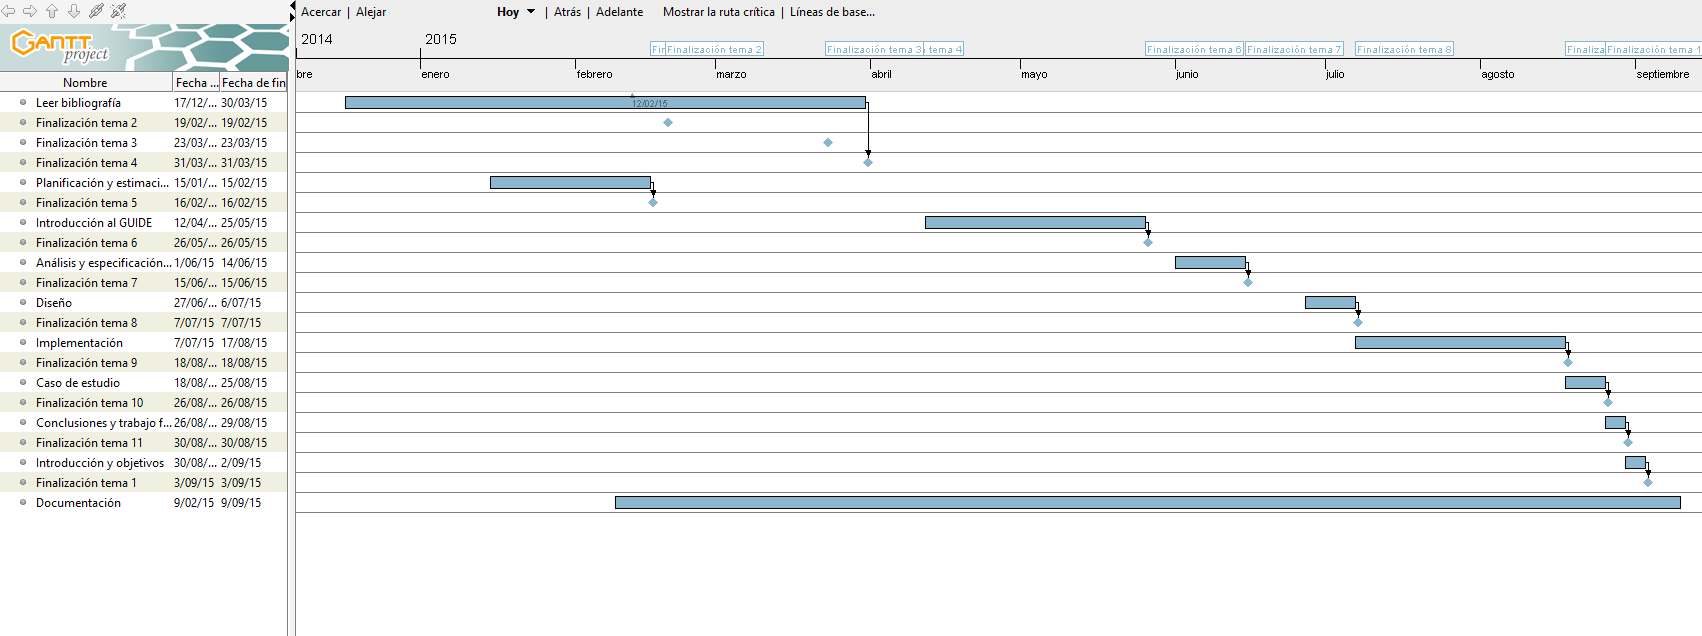
\includegraphics[width=1.8\textwidth]{imagenes/figuras/5_1.png}
\caption{Temporización en GanttProject.}
\end{figure}
\end{landscape}

\bigskip

Como se puede apreciar en la figura 5.1 la fase de documentación se hace en paralelo a cada una de las demás, puesto que el desarrollo de cada uno de los temas se van incluyendo en el documento final de forma progresiva.
Una estimación de las horas de trabajo dedicadas a cada fase aparece en la siguiente  tabla:

\bigskip
\begin{table}[htb]
\begin{center}
\begin{tabular}{|l|l|l|l|}
\hline
  & Días & Horas & Total \\
\hline \hline
Fase 1 & 104 & 2 & 208 \\ \hline
Fase 2 & 205 & 2 & 410 \\ \hline
Fase 3 & 66 &4 & 264 \\ \hline
Fase 4 & 8 & 6 & 40 \\ \hline
Fase 5 & 4 & 3 & 12 \\ \hline
Fase 6 & 6 & 6 & 36 \\ \hline
&&Tiempo total & 970 \\ \hline
\end{tabular}
\caption{Cálculo de horas de trabajo.}
\end{center}
\end{table}

\begin{figure}[H]
\centering
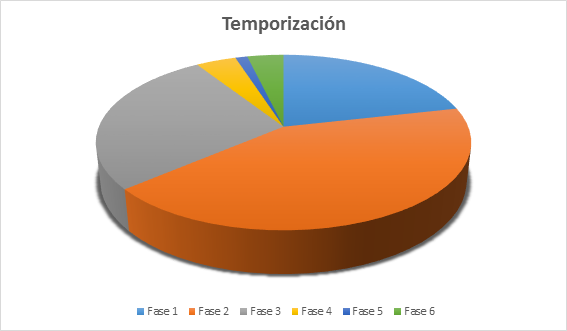
\includegraphics[width=0.9\textwidth]{imagenes/figuras/5_2.png}
\caption{Gráfico de la temporización.}
\end{figure}


\section{Recursos}
\subsection{Recursos humanos}

\begin{itemize}
\item D. José Camacho Páez, Profesor titular del departamento de Teoría de la señal, Telemática y comunaciones (TSTC) de la Universidad de Granada. Tutor del trabajo.
\item	Pablo Sánchez Robles, alumno de la Escuelta Técnica Superior de Ingeniería Informática y Telecomunicaciones (ETSIIT) de la Universidad de Granada. Autor del trabajo.
\end{itemize}
\bigskip
\subsection{Recursos hardware}
\begin{itemize}
\item Ordenador personal.
\end{itemize}

\bigskip

\subsection{Recursos software}

\begin{itemize}
\item Sistema operativo Windows 8.1.
\item Matlab® R2015a versión 8.5.
\item MEDA-Toolbox.
\item Evolus Pencil 2.0.5 (Diseño de interfaces gráficas)
\item ArgoUML 1.4	(Desarrollo de diagramas)
\item GanttProject 2.7.1	(Gráfico de temporización)
\item Texmaker	(Editor Latex)
\end{itemize}

\section{Estimación de costes}
\subsection{Herramientas hardware y software}
\begin{table}[htb]
\begin{center}
\begin{tabular}{|l|l|}
\hline
Recursos & Costes(Euros) \\
\hline \hline
Licencia Windows 8.1 & 138 \\ \hline
Matlab®(Student Version + toolboxes) & 321 \\ \hline
MEDA-Toolbox & 0 \\ \hline
Evolus Pencil & 0 \\ \hline
ArgoUML & 0 \\ \hline
GanttProject & 0 \\ \hline
Texmaker & 0 \\ \hline
Ordenador personal & 1200 \\ \hline
Total & 1659 \\ \hline
\end{tabular}
\caption{Costes herramientas.}
\end{center}
\end{table}

\bigskip
\begin{figure}[H]
\centering
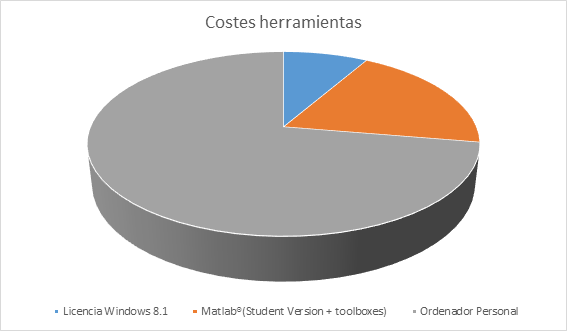
\includegraphics[width=0.9\textwidth]{imagenes/figuras/5_3.png}
\caption{Gráfico costes herramientas.}
\end{figure}
\bigskip

\subsection{Presupuesto}
Para el coste de los recursos humanos se ha hecho una estimación de 20 euros por hora trabajada por parte de Pablo Sánchez Robles y el coste del trabajo del tutor a 60 euros por hora, con una estimación de unas 50 horas de trabajo.

\bigskip

\begin{table}[htb]
\begin{center}
\begin{tabular}{|l|l|}
\hline
Concepto & Coste(Euros) \\
\hline \hline
Recursos humanos & 22400 \\ \hline
Herramientas & 1659 \\ \hline
Total & 24059 \\ \hline
\end{tabular}
\caption{Costes herramientas.}
\end{center}
\end{table}

\begin{figure}
\centering
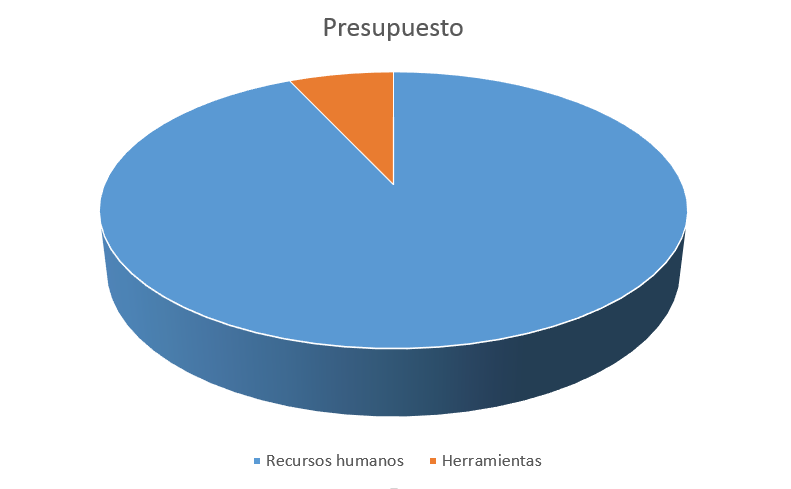
\includegraphics[width=0.9\textwidth]{imagenes/figuras/5_4.png}
\caption{Gráfico presupuesto total.}
\end{figure}

%
\chapter{GUIDE en Matlab} \cite{ML} \cite{MML}

\textbf{GUIDE}  son las siglas en ingles de “Graphic User Interfaze Development Environment”. Es un entorno de desarrollo de interfaces gráficas de usuario que proporciona MATLAB para facilitar la inserción de datos en aplicaciones por parte de los usuarios.
\bigskip

Esta herramienta se encarga de generar el código necesario para la creación de interfaces gráficas diseñadas en un entorno gráfico sin necesidad de una programación completa de las mismas, facilitando al programador el trabajo, que ya desarrolla el código vinculado a los eventos que se produzcan en la GUI.

\section{Componentes del entorno}

Para abrir el entorno en la consola de MATLAB se ejecuta el comando “guide” que muestra la pantalla de la figura 6.1.

\begin{figure}
\centering
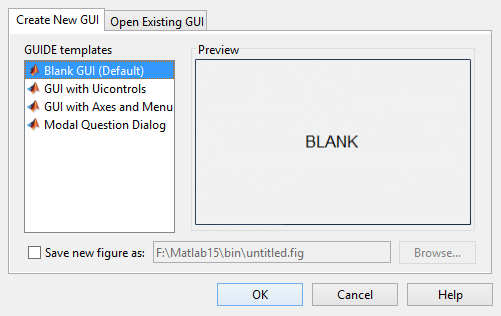
\includegraphics[width=0.9\textwidth]{imagenes/figuras/6_1.png}
\caption{Ventana incio GUIDE.}
\end{figure}

Las opciones que nos muestra son:

\begin{itemize}
\item \textbf{Blank GUI} crea una nueva interfaz en blanco para agregar los elementos que se deseen.
\item \textbf{GUI with UIcontrols} muestra un ejemplo de utilización de los controles de interfaz de usuario.
\item \textbf{GUI with Axes and Menu} muestra un ejemplo de interfaz con un menú desplegable para seleccionar un tipo de gráfico que se mostrará en el elemento Axes, que es un elemento de la GUI que sirve para proyectar gráficos de distintos tipos.
\item \textbf{Modal Question Dialog} muestra un ejemplo de interfaz con una pregunta que se puede responder con un sí o un no y según el botón pulsado devuelve una cosa u otra.
\end{itemize}

La opción más usual es Blank GUI para diseñar la interfaz deseada, mientras que las otras pueden servir de ejemplo para iniciarse en GUIDE. Una vez seleccionada dicha opción nos aparece la siguiente interfaz:


\begin{figure}[H]
\centering
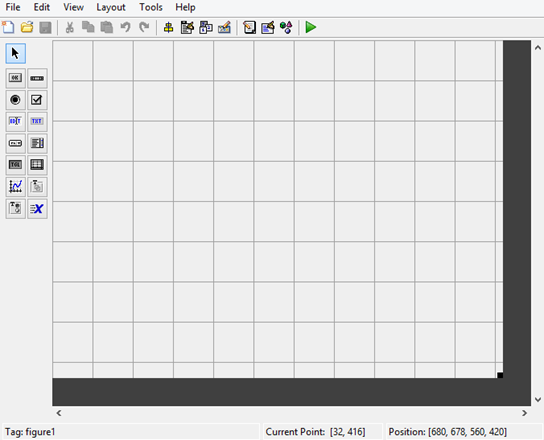
\includegraphics[width=0.9\textwidth]{imagenes/figuras/6_2.png}
\caption{GUIDE Blank GUI}
\end{figure}
\bigskip

Los elementos gráficos disponibles en GUIDE son:

\begin{table}[htb]
\begin{center}
\resizebox{10cm}{!} {
\begin{tabular}{|l|c|l|}
\hline
Elemento & Icono & Descripción \\
\hline \hline
Push Button&  
\includegraphics[width=0.05\textwidth]{imagenes/iconosguide/pushbuton.png} & Botón de una sola posición \\ \hline
Slider &
\includegraphics{imagenes/iconosguide/slider.png} & Barra deslizante \\ \hline
Radio Button&
\includegraphics{imagenes/iconosguide/radiobuton.png}  &Botón de selección única \\ \hline
Check Box&
\includegraphics{imagenes/iconosguide/check.png}   &Caaja de selección o botón de selección múltiple\\ \hline
Edit Text & 
\includegraphics{imagenes/iconosguide/edit.png} &Caja de texto editable  \\ \hline
Static Text& 
\includegraphics{imagenes/iconosguide/text.png} &Caja de texto no modificable  \\ \hline
Pop-up Menu& 
\includegraphics{imagenes/iconosguide/popup.png}  & Menú de selección desplegable\\ \hline
List Box&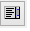
\includegraphics{imagenes/iconosguide/list.png}  &Lista delementos seleccionable \\ \hline
Toggle Button& 
\includegraphics{imagenes/iconosguide/togle.png}  &Botón de dos posiciones\\ \hline
Table&
\includegraphics{imagenes/iconosguide/table.png}   &Tabla numerada en filas y columnas\\ \hline
Axes&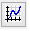
\includegraphics{imagenes/iconosguide/axes.png}   &Elemento para inserción de gráficos\\ \hline
Panel&
\includegraphics{imagenes/iconosguide/panel.png}  & Contenedor que puede reunir uno o varios elementos  \\ \hline
Button Group&
\includegraphics{imagenes/iconosguide/butongroup.png}   &Contenedor que agrupa Radio Buttons\\ \hline
ActiveX control&
\includegraphics{imagenes/iconosguide/activex.png}   &Contenedor de elementos ActiveX\\ \hline
\end{tabular}
}
\caption{Elementos de la interfaz gráfica.}
\end{center}
\end{table}
\bigskip

Cada uno de los elementos tiene una serie de propiedades modificables mediante el “property inspector”. Las propiedades más comunes a todos los elementos son el nombre (Tag), la posición en la que se encuentra dentro de la interfaz (Position), si está activo o no, si es visible o no y algunas relacionadas con el formato y tipo de fuente así como con la estética del elemento. En la figura 6.3 podemos ver un ejemplo de property inspector.
\bigskip

\begin{figure}
\centering
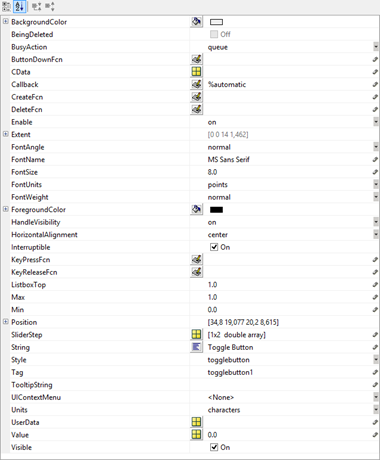
\includegraphics[width=0.6\textwidth]{imagenes/figuras/6_3.png}
\caption{Property Inspector.}
\end{figure}

Las demás propiedades son relativas al funcionamiento de cada elemento y no son comunes.
\bigskip

Otras opciones disponibles en GUIDE son las mostradas en la barra de herramientas(Tabla 6.2).

\begin{table}[H]
\begin{center}
\resizebox{12cm}{!} {
\begin{tabular}{|l|c|l|}
\hline
Herramienta & Icono & Descripción \\
\hline \hline
Nuevo&
\includegraphics{imagenes/iconosguide/nuevo.png} & Abre la ventana guide para crear nuevas interfaces \\ \hline
Abrir &
\includegraphics{imagenes/iconosguide/abrir.png} & Abre una interfaz anteriormente guardada \\ \hline
Guardar &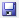
\includegraphics{imagenes/iconosguide/guardar.png} &Guarda la interfaz actual \\ \hline
Cortar&
\includegraphics{imagenes/iconosguide/cortar.png}  &Corta el elemento seleccionado\\ \hline
Copiar
\includegraphics{imagenes/iconosguide/copiar.png} & &Copia el elemento seleccionado\\ \hline
Pegar&
\includegraphics{imagenes/iconosguide/pegar.png} &Pega un elemento previamente cortado o copiado  \\ \hline
Atrás&
\includegraphics{imagenes/iconosguide/atras.png}  & Elimina el último cambio realizado en la interfaz\\ \hline
Adelante&
\includegraphics{imagenes/iconosguide/adelante.png} &Repone el paso previamente eliminado \\ \hline
Alinear&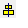
\includegraphics{imagenes/iconosguide/align.png}  &Abre un menú en el que se muestran distintos métodos de alineamiento de elementos del interfaz\\ \hline
Editor de menús &
\includegraphics{imagenes/iconosguide/menueditor.png} &Abre un entorno para la creación de menús\\ \hline
Inspector de propiedades&
\includegraphics{imagenes/iconosguide/propert.png}  &Abre el inspector de propiedades\\ \hline
Editor de pestañas &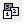
\includegraphics{imagenes/iconosguide/tabordereditor.png} &Abre una ventana para editar el orden de las distintas pestañas que tenga la interfaz\\ \hline
Editor de barras de herramientas&\includegraphics{imagenes/iconosguide/toolbareditor.png} &Abre un editor para la creación de barras de herramientas en la interfaz  \\ \hline
Editor&\includegraphics{imagenes/iconosguide/editor.png}  & Abre el código del elemento marcado\\ \hline
Buscador de objetos&\includegraphics{imagenes/iconosguide/object.png} &Muestra todos los elementos que maneja la interfaz para buscar uno en concreto \\ \hline
Run&\includegraphics{imagenes/iconosguide/run.png}  & Arranca la interfaz en modo ejecución\\ \hline
\end{tabular}
}
\caption{Herramientas disponibles en GUIDE.}
\end{center}
\end{table}
\bigskip

Una vez creada una nueva interfaz al darle a guardar genera dos ficheros uno de ellos “.fig” en el que se almacena los elementos gráficos del diseño y otro “.m” donde se inserta el código necesario para que funcione la misma.
\bigskip

Es dentro del fichero “.m” donde se tiene que añadir el código necesario para el funcionamiento de la aplicación. En dicho fichero insertaremos el código de los eventos de cada uno de los elementos de la interfaz, que en GUIDE se llaman “callbacks” y se añaden haciendo click con el botón derecho del ratón sobre el elemento concreto y en el menú desplegado pulsando en “View Callbacks” se muestran los distintos eventos que puede manejar el elemento seleccionado.
\bigskip

\section{Manejo desde código}

Para manejar cada uno de los elementos desde el código se utiliza el objeto hObject que se incluye como argumento de cada una de las llamadas a los métodos “callback” entre otros.
\bigskip

Dicho objeto sirve de contenedor, y para modificar cualquier dato se asigna a “handles” de la siguiente forma:
\bigskip

\textbf{handles.output = hObject;} 
\bigskip

Por ejemplo para tomar un elemento del interfaz gráfico se puede hacer:

\bigskip

\textbf{campo\_texto=get(handles.text1,’String’);}
\bigskip

Esto almacena en la variable campo\_texto el valor (Value) que tenga el campo de texto text1, para modificar el valor del mismo en el interfaz se debe  hacer con “set”:
\bigskip

\textbf{set(handles.text1,’String’, ‘Nuevo valor’);}
\bigskip

Con esta última sentencia se mostrara el texto “Nuevo valor” en el campo de texto text1 del interfaz.
\bigskip

En el caso de querer tomar los valores de “RadioButtons”, “Checkboxes”, “Lists”, etc, se tiene que hacer un get pero con el parámetro “Value” en lugar del “String”:
\bigskip

\textbf{Valor = get(handles.radio1,’Value’)}
\bigskip

La sentencia anterior devolverá 0 o 1 dependiendo si está o no marcado el radioButton radio1. Si en lugar de este tipo de elemento se tuviera una lista, ya sea desplegable o con slider, lo que devolvería “Value” seria la posición del elemento seleccionado de la lista.
\bigskip

\section{Ejemplo sencillo de interfaz con GUIDE}

En este apartado se va a mostrar un ejemplo sencillo de interfaz gráfica que mostrará un texto dentro de un campo de texto cuando se pulse un botón, el aspecto de la interfaz es:
\bigskip

\begin{figure}[H]
\centering
\includegraphics[width=0.9\textwidth]{imagenes/figuras/6_4.png}
\caption{Ejemplo de GUI, vista en GUIDE.}
\end{figure}
\bigskip

Esta es la vista desde GUIDE, la vista en ejecución es:
\bigskip

\begin{figure}[H]
\centering
\includegraphics[width=0.9\textwidth]{imagenes/figuras/6_5.png}
\caption{Ejemplo GUI, vista en ejecución.}
\end{figure}
\bigskip

La última vista es tras pulsar el botón:
\bigskip

\begin{figure}[H]
\centering
\includegraphics[width=0.9\textwidth]{imagenes/figuras/6_6.png}
\caption{Ejemplo GUI, vista tras pulsar el botón.}
\end{figure}
\bigskip

El código asociado al callback del botón es:
\bigskip

\begin{figure}[H]
\centering
\includegraphics[width=0.9\textwidth]{imagenes/figuras/6_7.png}
\caption{Código del callback.}
\end{figure}
\bigskip

Para un ejemplo más complejo del manejo de la interfaz desde el código ver el capítulo “implementación”.
%
\chapter{Análisis y especificación}

El análisis es la fase de la ingeniería del software en la que se describen las características necesarias para llevar a cabo los objetivos planteados en el software que se va a desarrollar. Previa a la fase del diseño sirve para descubrir los conflictos existentes entre requisitos y conocer más a fondo el sistema a desarrollar.
\bigskip

Para el desarrollo de todos los diagramas que aparecen en esta sección se ha utilizado ArgoUML, una aplicación de software libre que se puede encontrar en \cite{ARG}.
\bigskip

\section{Actores}
Son los entes que interactúan con el sistema, pueden ser personas, programas u otros sistemas remotos. En el caso que nos ocupa sólo hay un tipo de actor que sería el usuario:
\bigskip

\begin{itemize}
\item \textbf{Usuario:}Será la persona que utilice el software final para llevar acabo análisis de grandes conjuntos de datos. Está encuadrado en un público objetivo como pueden ser investigadores que necesiten encontrar patrones en grandes conjuntos de datos, administradores de redes que quieran detectar ataques en sus sistemas, etc. 
La materia que se estudie es irrelevante mientras los datos se estructuren como el software los acepta.
\end{itemize}
\bigskip

\subsection{Ficha de descripción de actor}

\begin{table}[H]
\begin{center}
\resizebox{10cm}{!} {
\begin{tabular}{|c|c|c|}
\hline
Actor & Usuario & Usr	\\ \hline
Descripción &\multicolumn{2}{|c|}{Actor encargado de utilizar el sistema}	\\ \hline
Características & \multicolumn{2}{|c|}{No existen características previas necesarias}	\\ \hline
Relaciones & \multicolumn{2}{|c|}{No posee relaciones con otros actores}	\\ \hline
Referencias &\multicolumn{2}{|c|}{CU-1,CU-2,CU-3,CU-4,CU-5,CU-6,CU-7}	\\ \hline
\end{tabular}
}
\caption{Ficha de descripción de usuarios.}
\end{center}
\end{table}

\bigskip

Cada uno de los elementos que aparecen en la sección "Referencias" son los casos de uso que se explicaran a lo largo del presente capítulo.

\section{Requisitos}
\bigskip

\subsection{Requisitos no funcionales}

Son restricciones que afectan a las funciones del software, acotando el diseño. No definen las funciones si no las propiedades.

\begin{itemize}
\item \textbf{RNF-1:}El sistema debe estar desarrollado en MATLAB.
\item \textbf{RNF-2:}El sistema debe hacer uso de “MEDA-Toolbox”.
\item \textbf{RNF-3:}El sistema debe ser portable y multiplataforma.
\item \textbf{RNF-4:}Los datos de entrada deben ser validados.
\item \textbf{RNF-5:}Los errores en la introducción de datos deben ser capturados y notificados.
\item \textbf{RNF-6:}Todo el software desarrollado debe ser libre y accesible a la comunidad.
\end{itemize}

\bigskip

\subsection{Requisitos funcionales}
Los requisitos funcionales son las características que debe poseer el sistema para llevar a cabo todos los objetivos planteados y cubrir las necesidades de los usuarios que lo utilicen.

\begin{itemize}
\item \textbf{RF-1:}Procesamiento de los datos a analizar.
\item \textbf{RF-2:}Generación de modelos completos con toda la información.
\item \textbf{RF-3:}Generación de modelos intermedios para cada fichero de datos.
\item \textbf{RF-4:}Almacenamiento de la información del entorno en ficheros.
\item \textbf{RF-5:}Generación de Score Plots, MEDA y oMEDA.
\item \textbf{RF-6:}Carga de entornos desde ficheros.
\end{itemize}

\bigskip

\subsection{Requisitos de información}

Los requisitos de información están relacionados con los datos que el sistema necesita almacenar para su funcionamiento. En el caso que nos ocupa el sistema no necesita almacenar datos para funcionar, aunque brinda la oportunidad de almacenar el entorno de trabajo para no tener que repetir tratamientos de los datos o análisis. 

\begin{itemize}
\item \textbf{RI-1:}El sistema sólo almacenará información ya tratada, los datos que se le pasen deben estar anonimizados y en ningún caso guardará información sensible.
\end{itemize}

\bigskip

\section{Casos de uso}

Se define caso de uso como la secuencia de interacciones que se dan entre los actores y el sistema. Se utilizan para guiar el diseño de la interfaz de usuario, facilitar la construcción de prototipos, son la base del diseño, lo validan y se pueden utilizar como base de los manuales de usuario.

\bigskip

\subsection{Fichas de descripción de los casos de uso}

\begin{table}[H]
\begin{center}
\resizebox{15cm}{!} {
\begin{tabular}{|c|c|c|c|}
\hline
\textbf{Caso de uso} &\multicolumn{2}{|c|}{Cargar fichero}  & CU-1	\\ \hline
\textbf{Actores} &\multicolumn{3}{|c|}{Usuario}	\\ \hline
\textbf{Tipo} & \multicolumn{3}{|c|}{Primario-Real}	\\ \hline
\textbf{Referencias} & \multicolumn{3}{|c|}{CU-2}	\\ \hline
\textbf{Precondición} &\multicolumn{3}{|c|}{Debe de existir el fichero a cargar y tener la estructura correcta}	\\ \hline
\textbf{Postcondición} &\multicolumn{3}{|c|}{No tiene}	\\ \hline
\textbf{Autor} & Pablo Sánchez Robles & \textbf{Versión} & 1.0\\ \hline
\multicolumn{4}{|c|}{\textbf{Propósito}}	\\ \hline
\multicolumn{4}{|c|}{Cargar el entorno desde un fichero	}\\ \hline
\multicolumn{4}{|c|}{\textbf{Resumen}}\\ \hline
\multicolumn{4}{|c|}{
  \begin{tabular}[c]{@{}l@{}}
	    Este caso de uso toma de un fichero el modelo o modelos\\
	   creados en una sesión anterior y los carga en el entorno de trabajo
	   \end{tabular}}\\ \hline
\end{tabular}
}
\caption{Ficha de CU-1.}
\end{center}
\end{table}

\begin{table}[H]
\begin{center}
\resizebox{15cm}{!} {
\begin{tabular}{|c|c|c|c|}
\hline
\textbf{Caso de uso} &\multicolumn{2}{|c|}{Guardar fichero}  & CU-2	\\ \hline
\textbf{Actores} &\multicolumn{3}{|c|}{Usuario}	\\ \hline
\textbf{Tipo} & \multicolumn{3}{|c|}{Primario-Real}	\\ \hline
\textbf{Referencias} & \multicolumn{3}{|c|}{CU-1}	\\ \hline
\textbf{Precondición} &\multicolumn{3}{|c|}{Debe de haber datos en el entorno de trabajo para poder guardar}	\\ \hline
\textbf{Postcondición} &\multicolumn{3}{|c|}{No tiene	}	\\ \hline
\textbf{Autor} & Pablo Sánchez Robles & \textbf{Versión} & 1.0\\ \hline
\multicolumn{4}{|c|}{\textbf{Propósito}}	\\ \hline
\multicolumn{4}{|c|}{Poder almacenar información en un fichero}\\ \hline
\multicolumn{4}{|c|}{\textbf{Resumen}}\\ \hline
\multicolumn{4}{|c|}{
Almacena el entorno de trabajo en un fichero}\\ \hline
\end{tabular}
}
\caption{Ficha de CU-2.}
\end{center}
\end{table}

\begin{table}[H]
\begin{center}
\resizebox{15cm}{!} {
\begin{tabular}{|c|c|c|c|}
\hline
\textbf{Caso de uso} &\multicolumn{2}{|c|}{Generar modelos completos}  & CU-3	\\ \hline
\textbf{Actores} &\multicolumn{3}{|c|}{Usuario}	\\ \hline
\textbf{Tipo} & \multicolumn{3}{|c|}{Primario-Real}	\\ \hline
\textbf{Referencias} & \multicolumn{3}{|c|}{No tiene}	\\ \hline
\textbf{Precondición} &\multicolumn{3}{|c|}{Tener acceso a los datos validados para el análisis}	\\ \hline
\textbf{Postcondición} &\multicolumn{3}{|c|}{No tiene}	\\ \hline
\textbf{Autor} & Pablo Sánchez Robles & \textbf{Versión} & 1.0\\ \hline
\multicolumn{4}{|c|}{\textbf{Propósito}}	\\ \hline
\multicolumn{4}{|c|}{Generar un solo modelo con todos los datos }\\ \hline
\multicolumn{4}{|c|}{\textbf{Resumen}}\\ \hline
\multicolumn{4}{|c|}{
\begin{tabular}[c]{@{}l@{}}
Crear una estructura de datos que almacene toda la\\
 información necesaria para el análisis
\end{tabular}
}\\ \hline
\end{tabular}
}
\caption{Ficha de CU-3.}
\end{center}
\end{table}

\begin{table}[H]
\begin{center}
\resizebox{15cm}{!} {
\begin{tabular}{|c|c|c|c|}
\hline
\textbf{Caso de uso} &\multicolumn{2}{|c|}{Generar modelos intermedios}  & CU-4	\\ \hline
\textbf{Actores} &\multicolumn{3}{|c|}{Usuario}	\\ \hline
\textbf{Tipo} & \multicolumn{3}{|c|}{Primario-Real}	\\ \hline
\textbf{Referencias} & \multicolumn{3}{|c|}{No tiene}	\\ \hline
\textbf{Precondición} &\multicolumn{3}{|c|}{Tener acceso a los datos validados para el análisis}	\\ \hline
\textbf{Postcondición} &\multicolumn{3}{|c|}{No tiene}	\\ \hline
\textbf{Autor} & Pablo Sánchez Robles & \textbf{Versión} & 1.0\\ \hline
\multicolumn{4}{|c|}{\textbf{Propósito}}	\\ \hline
\multicolumn{4}{|c|}{Generar un modelo por cada fichero de datos del estudio.}\\ \hline
\multicolumn{4}{|c|}{\textbf{Resumen}}\\ \hline
\multicolumn{4}{|c|}{
\begin{tabular}[c]{@{}l@{}}
Crear varias estructuras de datos que almacenen la información.\\
Una por cada fichero de datos conservando las características de cada uno.
\end{tabular}
}\\ \hline
\end{tabular}
}
\caption{Ficha de CU-4.}
\end{center}
\end{table}

\begin{table}[H]
\begin{center}
\resizebox{15cm}{!} {
\begin{tabular}{|c|c|c|c|}
\hline
\textbf{Caso de uso} &\multicolumn{2}{|c|}{Generar Score Plots}  & CU-5	\\ \hline
\textbf{Actores} &\multicolumn{3}{|c|}{Usuario}	\\ \hline
\textbf{Tipo} & \multicolumn{3}{|c|}{Primario-Real}	\\ \hline
\textbf{Referencias} & \multicolumn{3}{|c|}{CU-3 o CU-4}	\\ \hline
\textbf{Precondición} &\multicolumn{3}{|c|}{
\begin{tabular}[c]{@{}l@{}}
Debe existir al menos una estructura de datos \\
con la información tratada
\end{tabular}
}	\\ \hline
\textbf{Postcondición} &\multicolumn{3}{|c|}{No tiene	}	\\ \hline
\textbf{Autor} & Pablo Sánchez Robles & \textbf{Versión} & 1.0\\ \hline
\multicolumn{4}{|c|}{\textbf{Propósito}}	\\ \hline
\multicolumn{4}{|c|}{Generar un Score Plots y mostrarlo por pantalla}\\ \hline
\multicolumn{4}{|c|}{\textbf{Resumen}}\\ \hline
\multicolumn{4}{|c|}{
\begin{tabular}[c]{@{}l@{}}
Crea un Score Plots por cada estructura de datos que se 
\\tenga en el entorno de trabajo
\end{tabular}
}\\ \hline
\end{tabular}
}
\caption{Ficha de CU-5.}
\end{center}
\end{table}

\begin{table}[H]
\begin{center}
\resizebox{15cm}{!} {
\begin{tabular}{|c|c|c|c|}
\hline
\textbf{Caso de uso} &\multicolumn{2}{|c|}{Generar gráfica MEDA}  & CU-6	\\ \hline
\textbf{Actores} &\multicolumn{3}{|c|}{Usuario}	\\ \hline
\textbf{Tipo} & \multicolumn{3}{|c|}{Primario-Real}	\\ \hline
\textbf{Referencias} & \multicolumn{3}{|c|}{CU-3 o CU-4}	\\ \hline
\textbf{Precondición} &\multicolumn{3}{|c|}{
\begin{tabular}[c]{@{}l@{}}
Debe existir al menos una estructura de datos \\
con la información tratada
\end{tabular}
}	\\ \hline
\textbf{Postcondición} &\multicolumn{3}{|c|}{No tiene}	\\ \hline
\textbf{Autor} & Pablo Sánchez Robles & \textbf{Versión} & 1.0\\ \hline
\multicolumn{4}{|c|}{\textbf{Propósito}}	\\ \hline
\multicolumn{4}{|c|}{Generar una gráfica MEDA y mostrarla por pantalla}\\ \hline
\multicolumn{4}{|c|}{\textbf{Resumen}}\\ \hline
\multicolumn{4}{|c|}{
\begin{tabular}[c]{@{}l@{}}
Crea una matriz MEDA por cada estructura de datos que se tenga
\\ en el entorno de trabajo y la muestra por pantalla
\end{tabular}
}\\ \hline
\end{tabular}
}
\caption{Ficha de CU-6.}
\end{center}
\end{table}

\begin{table}[H]
\begin{center}
\resizebox{15cm}{!} {
\begin{tabular}{|c|c|c|c|}
\hline
\textbf{Caso de uso} &\multicolumn{2}{|c|}{Generar gráfica MEDA}  & CU-7	\\ \hline
\textbf{Actores} &\multicolumn{3}{|c|}{Usuario}	\\ \hline
\textbf{Tipo} & \multicolumn{3}{|c|}{Primario-Real}	\\ \hline
\textbf{Referencias} & \multicolumn{3}{|c|}{CU-5}	\\ \hline
\textbf{Precondición} &\multicolumn{3}{|c|}{Debe haberse generado previamente un Score Plots}	\\ \hline
\textbf{Postcondición} &\multicolumn{3}{|c|}{No tiene.}	\\ \hline
\textbf{Autor} & Pablo Sánchez Robles & \textbf{Versión} & 1.0\\ \hline
\multicolumn{4}{|c|}{\textbf{Propósito}}	\\ \hline
\multicolumn{4}{|c|}{Crear un gráfico oMEDA}\\ \hline
\multicolumn{4}{|c|}{\textbf{Resumen}}\\ \hline
\multicolumn{4}{|c|}{
\begin{tabular}[c]{@{}l@{}}
Generar y mostrar un gráfico oMEDA a partir de un Score Plots 
\\del que se seleccionan los puntos a incluir en oMEDA
\end{tabular}
}\\ \hline
\end{tabular}
}
\caption{Ficha de CU-7.}
\end{center}
\end{table}
\bigskip

\subsection{Curso normal de los casos de uso}

\bigskip
\begin{table}[H]
      \begin{center}
	\begin{tabular}{|l|l|l|l|}
	  \hline
	  \multicolumn{4}{|c|}{{\bf Curso normal}}
	  \\ \hline
	  \multicolumn{2}{|c|}{{\bf Actor}} & \multicolumn{2}{c|}{{\bf Sistema}}
	  \\ \hline
	  {\it 1} & 
	  \begin{tabular}[c]{@{}l@{}}
	    Usuario: Ordenar carga\\
	    de un fichero guardado.\\
	  \end{tabular} &
	  &
	  \\ \hline
	  &
	  &
	  {\it 2} &
	  \begin{tabular}[c]{@{}l@{}}
	   Cargar entorno con los datos\\
	   del fichero.
	   \end{tabular}
	  \\ \hline
	\end{tabular}
	\caption{Curso normal de CU-1.}
      \end{center}
    \end{table}
    
  \begin{table}[H]
      \begin{center}
	\begin{tabular}{|l|l|l|l|}
	  \hline
	  \multicolumn{4}{|c|}{{\bf Curso normal}}
	  \\ \hline
	  \multicolumn{2}{|c|}{{\bf Actor}} & \multicolumn{2}{c|}{{\bf Sistema}}
	  \\ \hline
	  {\it 1} & 
	  \begin{tabular}[c]{@{}l@{}}
	    Usuario: Ordenar guardado \\
	    del entorno en un fichero.\\
	  \end{tabular} &
	  &
	  \\ \hline
	  &
	  &
	  {\it 2} &
	  \begin{tabular}[c]{@{}l@{}}
	   Guardar los datos actuales \\
	   en el fichero indicado.\\
	   \end{tabular}
	  \\ \hline
	\end{tabular}
	\caption{Curso normal de CU-2.}
      \end{center}
    \end{table}  
    
    \begin{table}[H]
      \begin{center}
	\begin{tabular}{|l|l|l|l|}
	  \hline
	  \multicolumn{4}{|c|}{{\bf Curso normal}}
	  \\ \hline
	  \multicolumn{2}{|c|}{{\bf Actor}} & \multicolumn{2}{c|}{{\bf Sistema}}
	  \\ \hline
	  {\it 1} & 
	  \begin{tabular}[c]{@{}l@{}}
	   Usuario: proporcionar los \\
	   datos necesarios para el \\
	   análisis y ordenar generar\\
	    un modelo con ellos.
	  \end{tabular} &
	  &
	  \\ \hline
	  &
	  &
	  {\it 2} &
	  \begin{tabular}[c]{@{}l@{}}
	   Validar los datos proporcionados.\\
	   \end{tabular}
	  \\ \hline
	   &
	   &
	   {\it 3} &
	  \begin{tabular}[c]{@{}l@{}}
	 Generar una estructura de \\
	 datos con los resultados \\
	 del análisis.
	   \end{tabular}
	   \\ \hline
	\end{tabular}
	\caption{Curso normal de CU-3.}
      \end{center}
    \end{table}  
    \newpage
    \begin{table}[H]
      \begin{center}
	\begin{tabular}{|l|l|l|l|}
	  \hline
	  \multicolumn{4}{|c|}{{\bf Curso normal}}
	  \\ \hline
	  \multicolumn{2}{|c|}{{\bf Actor}} & \multicolumn{2}{c|}{{\bf Sistema}}
	  \\ \hline
	  {\it 1} & 
	  \begin{tabular}[c]{@{}l@{}}
	   Usuario: proporcionar los \\
	   datos necesarios para el \\
	   análisis y ordenar generar\\
	    los modelos intermedios.
	  \end{tabular} &
	  &
	  \\ \hline
	  &
	  &
	  {\it 2} &
	  \begin{tabular}[c]{@{}l@{}}
	   Validar los datos proporcionados.\\
	   \end{tabular}
	  \\ \hline
	   &
	   &
	   {\it 3} &
	  \begin{tabular}[c]{@{}l@{}}
		Generar estructuras de datos\\
		intermedias con los resultados\\
		del análisis
	 del análisis.
	   \end{tabular}
	   \\ \hline
	\end{tabular}
	\caption{Curso normal de CU-4.}
      \end{center}
    \end{table}  
    
    \begin{table}[H]
      \begin{center}
	\begin{tabular}{|l|l|l|l|}
	  \hline
	  \multicolumn{4}{|c|}{{\bf Curso normal CU-5}}
	  \\ \hline
	  \multicolumn{2}{|c|}{{\bf Actor}} & \multicolumn{2}{c|}{{\bf Sistema}}
	  \\ \hline
	  {\it 1} & 
	  \begin{tabular}[c]{@{}l@{}}
	  Usuario: Ordenar la generación\\
	  de Score Plots.
	  \end{tabular} &
	  &
	  \\ \hline
	  &
	  &
	  {\it 2} &
	  \begin{tabular}[c]{@{}l@{}}
	   Comprobar que existe al menos\\
	    una estructura de datos con \\
	    información procesada para\\
	    poder generar la gráfica.
	   \end{tabular}
	  \\ \hline
	   &
	   &
	   {\it 3} &
	  \begin{tabular}[c]{@{}l@{}}
	   Generar un Score Plots por\\
	   cada estructura de datos completa.
	   \end{tabular}
	   \\ \hline
	\end{tabular}
	\caption{Curso normal de CU-5.}
      \end{center}
    \end{table}  
    
    \begin{table}[H]
      \begin{center}
	\begin{tabular}{|l|l|l|l|}
	  \hline
	  \multicolumn{4}{|c|}{{\bf Curso normal CU-6}}
	  \\ \hline
	  \multicolumn{2}{|c|}{{\bf Actor}} & \multicolumn{2}{c|}{{\bf Sistema}}
	  \\ \hline
	  {\it 1} & 
	  \begin{tabular}[c]{@{}l@{}}
	   Usuario: Ordenar la generación \\
	   de gráfica MEDA.
	  \end{tabular} &
	  &
	  \\ \hline
	  &
	  &
	  {\it 2} &
	  \begin{tabular}[c]{@{}l@{}}
	  Comprobar que existe al menos\\ 
	  una estructura de datos con\\
	  información procesada para\\
	  poder generar la gráfica.
	   \end{tabular}
	  \\ \hline
	   &
	   &
	   {\it 3} &
	  \begin{tabular}[c]{@{}l@{}}
	 Generar un gráfico MEDA \\
	 con la estructura seleccionada.
	   \end{tabular}
	   \\ \hline
	\end{tabular}
	\caption{Curso normal de CU-6.}
      \end{center}
    \end{table} 
     
    \newpage
    \begin{table}[H]
      \begin{center}
	\begin{tabular}{|l|l|l|l|}
	  \hline
	  \multicolumn{4}{|c|}{{\bf Curso normal CU-7}}
	  \\ \hline
	  \multicolumn{2}{|c|}{{\bf Actor}} & \multicolumn{2}{c|}{{\bf Sistema}}
	  \\ \hline
	  {\it 1} & 
	  \begin{tabular}[c]{@{}l@{}}
	   Usuario: Seleccionar Puntos \\
	   deseados del Score Plots,\\
	   ordenar la generación de la \\
	   gráfica oMEDA con dichos puntos.
	  \end{tabular} &
	  &
	  \\ \hline
	  &
	  &
	  {\it 2} &
	  \begin{tabular}[c]{@{}l@{}}
	  Comprobar que se han \\
	  seleccionado puntos\\
	   de un Score Plots.
	   \end{tabular}
	  \\ \hline
	   &
	   &
	   {\it 3} &
	  \begin{tabular}[c]{@{}l@{}}
	 Generar un gráfico oMEDA con\\
	 los puntos seleccionados \\
	 del Score Plots.
	   \end{tabular}
	   \\ \hline
	\end{tabular}
	\caption{Curso normal de CU-7.}
      \end{center}
    \end{table}  
    
\subsection{Cursos alternos de los casos de uso}
\bigskip

\begin{table}[H]
    \begin{center}
	\begin{tabular}{|l|l|l|l|}
	  \hline
	  \multicolumn{4}{|c|}{{\bf Curso alterno CU-5}}
	  \\ \hline
	  \multicolumn{2}{|c|}{{\bf Actor}} & \multicolumn{2}{c|}{{\bf Sistema}}
	  \\ \hline
	  & &
	  {\it 1} & 
	  \begin{tabular}[c]{@{}l@{}}
	    Si no existe ninguna estructura\\
	    de datos con información mostrar\\
	    mensaje y cancelar procedimiento.
	  \end{tabular} 
	  \\ \hline
	\end{tabular}
	\caption{Curso alterno de CU-5.}
     \end{center}
\end{table}

\begin{table}[H]
    \begin{center}
	\begin{tabular}{|l|l|l|l|}
	  \hline
	  \multicolumn{4}{|c|}{{\bf Curso alterno CU-6}}
	  \\ \hline
	  \multicolumn{2}{|c|}{{\bf Actor}} & \multicolumn{2}{c|}{{\bf Sistema}}
	  \\ \hline
	  & &
	  {\it 1} & 
	  \begin{tabular}[c]{@{}l@{}}
	   Si no existe ninguna estructura\\
	    de datos con información mostrar\\
	     mensaje y cancelar procedimiento.
	  \end{tabular} 
	  \\ \hline
	\end{tabular}
	\caption{Curso alterno de CU-6.}
     \end{center}
\end{table}

\begin{table}[H]
    \begin{center}
	\begin{tabular}{|l|l|l|l|}
	  \hline
	  \multicolumn{4}{|c|}{{\bf Curso alterno CU-7}}
	  \\ \hline
	  \multicolumn{2}{|c|}{{\bf Actor}} & \multicolumn{2}{c|}{{\bf Sistema}}
	  \\ \hline
	  & &
	  {\it 1} & 
	  \begin{tabular}[c]{@{}l@{}}
	   Si no se han seleccionado puntos\\
	   de un Score Plots mostrar\\
	    mensaje y cancelar 
	   \\procedimiento.
	  \end{tabular} 
	  \\ \hline
	\end{tabular}
	\caption{Curso alterno de CU-7.}
     \end{center}
\end{table}

\subsection{Diagramas de casos de uso}

Representan de forma visual las relaciones entre los actores y sus casos de uso asociados.

\begin{figure}[H]
\centering
\includegraphics[width=0.9\textwidth]{imagenes/diagramas/DCU1.png}
\caption{Diagrama de casos de uso Análisis-Calibración.}
\end{figure}
\
\begin{figure}[H]
\centering
\includegraphics[width=0.9\textwidth]{imagenes/diagramas/DCU2.png}
\caption{Diagrama de casos de uso Visualización.}
\end{figure}
\newpage
\section{Diagrama de paquetes}

Este tipo de diagrama representa la estructura según las relaciones lógicas existentes así como las dependencias entre los elementos que componen el software. Cada paquete nos sirve como estructura para organizar ciertos elementos del modelo agrupándolos.
\bigskip

\begin{figure}[H]
\centering
\includegraphics[width=0.9\textwidth]{imagenes/diagramas/DDP.png}
\caption{Diagrama de paquetes.}
\end{figure}

Se puede observar en el diagrama de paquetes que el paquete “Analyze” depende del “Model Calibration” lo cual quiere decir que para poder analizar los datos primero se debe calibrar el modelo mediante los parámetros de entrada. Por otra parte para poder llevar a cabo la visualización se tienen que tener los datos ya calibrados y analizados,  almacenados en una estructura de datos. Como vemos todo el conjunto de paquetes GUI-BIGDATA depende de MEDA-Toolbox que para simplificar el diagrama ha sido encapsulada en un solo paquete.
\bigskip

\section{Diagramas de actividad}

Este tipo de diagramas representan la actividad de un caso de uso, la actividad realizada por un conjunto de objetos o los flujos entre varios casos de uso.
\bigskip

Para los dos primeros casos de uso los diagramas de actividad son triviales puesto que tanto para guardar como para cargar ficheros se selecciona un fichero concreto, lo cual hace el diagrama innecesario.
\bigskip

\begin{figure}[H]
\centering
\includegraphics[width=0.9\textwidth]{imagenes/diagramas/DA1.png}
\caption{Diagrama de actividad CU-3.}
\end{figure}

\begin{figure}[H]
\centering
\includegraphics[width=0.9\textwidth]{imagenes/diagramas/DA2.png}
\caption{Diagrama de actividad CU-4.}
\end{figure}

\begin{figure}[H]
\centering
\includegraphics[width=0.9\textwidth]{imagenes/diagramas/DA3.png}
\caption{Diagrama de actividad CU-5.}
\end{figure}

\begin{figure}[H]
\centering
\includegraphics[width=0.9\textwidth]{imagenes/diagramas/DA4.png}
\caption{Diagrama de actividad CU-6.}
\end{figure}


\begin{figure}[H]
\centering
\includegraphics[width=0.9\textwidth]{imagenes/diagramas/DA5.png}
\caption{Diagrama de actividad CU-7.}
\end{figure}

%
\chapter{Diseño}

En este apartado se van a describir cada una de las herramientas, entornos y metodologías que se van a seguir a la hora de implementar el software del que se ha hecho el análisis y especificación en el capítulo anterior.
\bigskip

\section{Herramientas a utilizar}

Para el desarrollo se va a utilizar el lenguaje de programación M propio de MATLAB cuyo núcleo está desarrollado en C y Java. Es de propósito específico para la implementación de software matemático, que con el tiempo ha ido ampliando sus capacidades de desarrollo hasta convertirse en un lenguaje completo que puede crear interfaces gráficas mediante GUIDE, interconexión con dispositivos hardware, etc.
\bigskip

Cómo se ha comentado en capítulos anteriores se va a hacer uso de la toolbox MEDA que implementa una serie de herramientas estadísticas para el análisis exploratorio de datos y la visualización de los mismos en distintos tipos de gráficas. Dicha toolbox tiene la capacidad de análisis supervisados de datos con PLS, análisis no supervisados con PCA y las visualizaciones se hacen mediante Score plots, Loading Plots, gráficos Meda y oMEDA.
\bigskip

Dentro de MEDA-Toolbox para este proyecto se van a utilizar los módulos:
\bigskip

\begin{itemize}
	\item \textbf{Update\_iterative2.m:} Se encarga de generar la estructura Lmodel mediante análisis PCA o PLS según se le especifique, siguiendo el método "iterative" para BIG DATA. Es una modificación del módulo update\_iterative.m añadiendo una funcionalidad de salida de información mediante una consola o terminal propio de cada interfaz gráfica que se le pasa por argumento al módulo.
	\item \textbf{Update\_ewma2.m:} Hace lo mismo que el módulo anterior pero basándose
en el método EWMA, al igual que en el caso anterior es una modificación de update\_ewma.m para añadir la funcionalidad de la consola propia.
	\item \textbf{Score\_LPLS.m:} Generar un gráfico Score Plots con BIG DATA y siguiendo el modelo PLS.
	\item \textbf{Scores\_LPCA.m:} Generar un gráfico Score Plots con BIG DATA y siguiendo el modelo PCA.
	\item \textbf{Meda\_LPLS.m:} Genera una matriz MEDA y la muestra por pantalla siguiendo el modelo PLS.
	\item \textbf{Meda\_LPCA.m:} Genera una matriz MEDA y la muestra por pantalla siguiendo el modelo PCA.
	\item \textbf{Omeda\_LPLS:} Genera un gráfico oMEDA siguiendo el modelo PLS con unos puntos seleccionados de un gráfico Score Plots.
	\item \textbf{Omeda\_LPCA:} Genera un gráfico oMEDA siguiendo el modelo PCA con unos puntos seleccionados de un gráfico Score Plots.
\end{itemize}

\section{Diseño de la interfaz}

Para el diseño de un prototipo de la GUI se va a utilizar la herramienta "Pencil Project" de código abierto que se puede encontrar en \cite{PE}. Con dicha herramienta se crean de forma sencilla estructuras similares a lo que sería la GUI final. Sirve para poder llevar un esquema de lo que se quiere hacer.

\bigskip

El prototipo diseñado para la interfaz gráfica de usuario es:

\begin{figure}[H]
\centering
\includegraphics[width=0.7\textwidth]{imagenes/figuras/8_1.png}
\caption{Prototipo de la GUI.}
\end{figure}

\bigskip

En la etapa de análisis y especificación se pensó en una estructura con 3 paquetes o módulos diferentes que dependían unos de otros, pero para el desarrollo de la GUI se han aunado en una sola interfaz facilitando la comprensión por parte del usuario. Aun así siguen estando separadas las funciones de calibración del modelo, análisis y visualización mediante paneles separadores. El prototipo consta de diferentes subsecciones, que son la entrada de datos en la parte superior, la entrada de atributos para calibración del modelo a analizar en la parte intermedia izquierda, la consola de
salida en la parte intermedia derecha y las características de la visualización
en la parte inferior.
\bigskip

\section{Diseño de la arquitectura}

La integración de los 3 paquetes de la fase de análisis en uno sólo se ha hecho por simplicidad en el código ya que M no es el mejor lenguaje de programación para aplicar el paradigma de la orientación a objetos. La estructura de 3 paquetes se integró para separar las 3 partes conceptuales de la aplicación ya que los procesos que implican cada una de ellas son diferentes aunque dependan unos de otros. Como la estructura de datos que utilizan los 3 módulos es la misma, un Lmodel, no tendría tampoco mucho sentido crear 3 clases diferentes ya que lo único que las diferenciaría sería la función principal de cada una. Por lo tanto cada uno de los paquetes de la etapa de análisis se va a transformar en un módulo funcional y no en una clase propia, y todos ellos estarían integrados en un mismo fichero, compartiendo todos los datos del entorno de trabajo sin la necesidad de establecer mecanismos de transmisión de datos entre ellos más allá de la generación de variables globales.
\bigskip

\section{Diseño de los ficheros de código}
Se crearán dos ficheros para el desarrollo del software: GuiV1.fig y GuiV1.m.

\begin{itemize}
\item \textbf{Guiv1.fig:} contendrá la estructura de la interfaz gráfica. Como se explicó en capítulos anteriores GUIDE genera este tipo de ficheros para almacenar toda la parte de la GUI relacionada con la estética.
\item \textbf{Guiv1.m:} Este fichero tendrá almacenado todo el código propiamente dicho de la aplicación, tanto la integración con la interfaz gráfica como los métodos que le dan funcionalidad al programa.
\end{itemize}
\bigskip

\section{Diseño de los ficheros de datos para las pruebas}

Como lo que se desea analizar es BIG DATA la extensión de los ficheros de datos puede llegar a alcanzar un tamaño demasiado grande para los tamaños de ficheros de los sistemas (sobre todo en sistemas operativos de 32 bits), además la función load de Matlab saturaría la RAM con ficheros muy grandes, por lo que los ficheros de datos propiamente dichos se van a dividir en varios de tamaño más pequeño y se van a indexar con otro tipo de fichero. Por lo tanto se tendrán dos tipos de ficheros:

\bigskip

\begin{itemize}
\item \textbf{Ficheros de datos:} Almacenarán dos matrices, una bidimensional con los valores de X y otra unidimensional con los valores de las clases de cada una de las observaciones. Si es un modelo PLS también contendrá la matriz Y. Opcionalmente se pueden tener matrices con las observaciones y nombre de las variables.
\item \textbf{Ficheros índice:} Deberán tener al menos una matriz unidimensional con las rutas a cada uno de los ficheros de datos, y como parte opcional se puede añadir otra con los nombres de las variables a analizar.

\end{itemize}
%
\chapter{Implementación}
Como se ha comentado en capítulos anteriores la implementación del software se ha desarrollado en el lenguaje de programación M, propio de Matlab y con el entorno de creación de interfaces de usuario GUIDE.

\bigskip

\section{Implementación de la interfaz gráfica}

Finalmente la GUI creada sigue los patrones estéticos diseñados en el capítulo anterior con pequeñas modificaciones para una mayor claridad y la inclusión de dos nuevos campos en la sección de visualización.

\begin{figure}[H]
\centering
\includegraphics[width=0.7\textwidth]{imagenes/figuras/9_1.png}
\caption{GUI final.}
\end{figure}

\bigskip

Como se puede observar en la figura 9.1 los cambios introducidos con respecto al diseño son mínimos, simplemente se han añadido unas etiquetas en cada uno de los paneles separadores identificando qué se hace dentro de cada uno de ellos, y unos botones de guardado del entorno y de carga de entornos guardados con anterioridad, además de dos menús desplegables para la selección de las componentes principales a visualizar.

\begin{figure}
\centering
\includegraphics[width=0.9\textwidth]{imagenes/figuras/9_2.png}
\caption{Ruta a los datos.}
\end{figure}

\bigskip

La figura 9.2 muestra la zona de la GUI donde se selecciona el conjunto de datos a analizar de un fichero “.mat”.

\begin{figure}
\centering
\includegraphics[width=0.9\textwidth]{imagenes/figuras/9_3.png}
\caption{Calibración del modelo.}
\end{figure}

\bigskip

En la figura 9.3 se puede ver la zona central de la interfaz, que aúna el módulo funcional de calibración del modelo con el de análisis, aunque como se verá más adelante en el código están separadas en dos funciones independientes.

\bigskip

Cada uno de los campos de la subsección “Variables” se explicaron con anterioridad en el capítulo 3.
\bigskip

En la subsección “Console” irán apareciendo todas las salidas que mostraría la aplicación al ejecutarse por terminal. 

\begin{figure}
\centering
\includegraphics[width=0.9\textwidth]{imagenes/figuras/9_4.png}
\caption{Visualización.}
\end{figure}

\bigskip

En la figura 9.4 se puede ver la subsección de “Visualization”, en la que se mostraran los modelos ya calibrados y estructurados mediantes los análisis correspondientes para poder visualizarlos en Score Plots, MEDA y oMEDA. El apartado oMEDA permite seleccionar los puntos a mostrar en el gráfico. Este apartado fué desarrollado por Elena Jimenez Mañas \cite{PHPDAT} y en el presente trabajo se ha adaptado para el manejo de Big Data. Los campos From y To son para seleccionar desde qué componente a qué otro se desea visualizar.


\section{Código desarrollado}

En esta sección se va a explicar el código desarrollado para los módulos comentados en la fase de diseño. Como se dijo anteriormente la fase de calibración del modelo y la de análisis se han fusionado en lo que a interfaz gráfica se refiere, pero el código de ambas funciones está separado.

\bigskip

La función \textbf{modelCalibration} se encarga de comprobar que todos los campos introducidos en la sección del mismo nombre de la GUI sean correctos y almacena los necesarios en variables globales para su uso continuo. Si alguno  de los campos no tiene valor lanza un mensaje de error pidiendo que se rellene para poder seguir adelante.
\bigskip

Tras confirmar que todos los campos han sido rellenados pasa a incializar el primero modelo con los datos proporcionados por el usuario y por último rellena las listas From y To del apartado Visualization con los componentes principales generados en función del campo Lvs.
\bigskip


la función \textbf{Analize}, comienza tomando las variables globales necesarias para llevar a cabo las tareas que se tienen que desarrollar en la misma, rellenas ya con los valores necesarios en modelCalibration.

\bigskip

A continuación se carga el fichero de datos introducido en la sección Data set Path, y según los campos seleccionados de la zona Model calibration de la GUI se va generando el primero modelo, a partir del cuál se generarán los demás si se ha seleccionado la opción Generate intermediate models, o se generará sólo ese si no se ha seleccionado dicha opción.

\bigskip

Si se ha seleccionado la opción Generate intermediate models se pasa a crear una lista con los nombres que se le van a dar a cada uno de los modelos, que cuando se termine el proceso aparecerá en el listboxModels del apartado de Visualization para poder seleccionar el que se desee para su visualización.

\bigskip

Una vez hecho esto se actualiza el primer modelo con la funcion update\_iterative2 o update\_ewma2 en función de la opción seleccionada en Model Calibration y a continuación se entra en un bucle que irá generando tantos modelos como ficheros de datos se tengan. Cada modelo se genera en función del anterior por ello el bucle comienza en 2 y termina en el tamaño de la lista que contenga el fichero índice.

\bigskip

En caso de que se quiera generar un sólo modelo el código es mas simple, sólo se toman los campos necesarios de las variables globales y se actualiza el modelo en función de las opciones seleccionadas.
\bigskip

La función \textbf{Visualize} se encarga de tomar los modelos generados y visualizar el que se ha seleccionado mediante las gráficas elegidas.

\bigskip

En primer lugar esta función toma la lista de modelos globales, a continuación comprueba que los campos From y To no tengan el mismo valor, y en caso de ser así lanza un mensaje de error y cancela la visualización.Tras esto compara los valores de From y To para almacenar el menor y el mayor de los componentes principales de la selección para así poder llevar a cabo la visualización correctamente cuando son listas de componentes múltiples.Después comprueba que exista mas de un modelo para poder seleccionar de la lista, y en caso de no ser así marca como seleccionado el único que hay.

\bigskip

Una vez hecho todo lo anterior se pasa a generar las gráficas en función del los campos seleccionados en la sección visualization. Si se ha elegido crear un scoreplot se almacenaran las salidas que produzca este (matrices de puntos) en la variable T para su posterior utilización en oMEDA, se marcará cada gráfica con el tag ScorePlot para poder identificarlo y se llamará a la función \textbf{preparaOmeda}. Por último si se ha marcado MEDA también se generará.
\bigskip

La función \textbf{preparaOmeda} se encarga de inicializar una serie de variables que se utilizarán para poder localizar los puntos que se seleccionarán del ScorePlot para generar el oMEDA. Esta función forma parte del código desarrollado por Elena Jiménez Mañas y no se ha modificado nada en el presente trabajo.

\bigskip

Las funciones asociadas a los eventos de pulsación de todos los botones de la subsección oMEDA fueron desarrolladas y explicadas en el PFC "Herramientas para la detección de ataques en tráfico de red" de Elena Jiménez Mañas.
%
\chapter{Caso de estudio}

En este capítulo se va a realizar un ejemplo de uso de la interfaz para la detección de anomalías en red con unos datos previamente anonimizados de una red corporativa real.

\bigskip

Primero se comenzará a hacer un análisis de todos los ficheros de datos como un único modelo y posteriormente en modelos separados de cada uno de los mismos. La figura 10.1 muestra la configuración utilizada para el primer análisis.

\bigskip

\begin{figure}[H]
\centering
\includegraphics[width=0.7\textwidth]{imagenes/casoEstudio/10_1.png}
\caption{GUI para un solo modelo.}
\end{figure}

\begin{figure}[!ht]
\centering
\includegraphics[width=0.7\textwidth]{imagenes/casoEstudio/10_2.png}
\caption{Score plot un modelo.}
\end{figure}

\bigskip

En la figura 10.2 se puede apreciar cómo hay varias observaciones que se salen de la concentración normal de datos, estos \textbf{outliers} pueden darnos información sobre una posible anomalía en el funcionamiento normal de la red.

\begin{figure}[H]
\centering
\includegraphics[width=0.7\textwidth]{imagenes/casoEstudio/10_3.png}
\caption{MEDA un modelo.}
\end{figure}

\bigskip

Las observaciones 65, 91, 48, 79 y 12 parecen no estar dentro de los "limites" que siguen el resto de las mismas, por lo que se van a estudiar más en profundidad. Para esto en el gráfico MEDA de la figura 10.3 se observa en términos generales el funcionamiento de la red, viendo las relaciones existentes entre variables. Posteriormente con oMEDA se verán las relaciones entre variables y observaciones.

\begin{figure}[!ht]
\centering
\includegraphics[width=0.7\textwidth]{imagenes/casoEstudio/10_4.png}
\caption{MEDA un modelo con zoom.}
\end{figure}

\bigskip

En la figura 10.4 se puede ver el gráfico MEDA ampliado en la zona donde existen relaciones para poder ver qué variables son las relacionadas. En Dicha figura se pueden observar las relaciones existentes entre variables quedando fuertemente relacionadas 4 grupos de variables. El primer grupo son las variables 80, 76 y 89. El segundo grupo son las variables 88, 75 y 79. El tercero las variables 36 y 1. Y el último 68 y 65. El contenido de las variables se muestra en la tabla 10.1. El primero de los 3 grupos mostrados en la tabla nos indica que en conexiones con paquetes de datos de gran tamaño el estado de la conexión se mantiene abierto durante todo el periodo de tiempo que ha durado la captura. El segundo muestra que en términos generales cuando los paquetes son de tamaño medio la conexión se cierra dentro del periodo de captura. El tercero nos dice que cuando el puerto de origen es privado la IP también lo es.

\begin{table}[H]
\begin{center}
\begin{tabular}{|c|c|c|}
\hline
\textbf{Variable} &\textbf{Nombre} & \textbf{Descripción} \\
 \hline \hline

89 & nf\_state\_open & Estado de conexión abierta	\\ \hline
80 & nf\_dbyte\_long & Paquetes de destino de gran tamaño \\ \hline
76 & nf\_sbyte\_long & Paquetes de origen de gran tamaño  \\	
\hline \hline

88 & nf\_state\_close & Estado de conexión cerrada	\\ \hline
79 & nf\_dbyte\_medium & Paquetes de destino de tamaño medio	\\ \hline
75 & nf\_sbyte\_medium & Paquetes de origen de tamaño medio\\
 \hline \hline

36 & nf\_sport\_private & Puerto de origen privado\\ \hline
1 & nf\_sip\_private & IP privada de origen	\\
\hline \hline

68 & nf\_dport\_register & Puerto de destino mayor a 1024\\ \hline 
65 & nf\_dport\_8089 & Puerto de destino 8089 \\ \hline 
\end{tabular}
\caption{Contenido variables.}
\end{center}
\end{table}

\bigskip

Ahora que ya se conoce el contenido de las variables mas relacionadas se pasa a crear un gráfico oMEDA con los outliers para poder relacionar variables con observaciones y poder encontrar dónde se producen las anomalías. En la figura 10.5 se ve como se marcan las observaciones outliers.

\begin{figure}
\centering
\includegraphics[width=0.7\textwidth]{imagenes/casoEstudio/10_5.png}
\caption{Observaciones marcadas para oMEDA.}
\end{figure}

\begin{figure}[H]
\centering
\includegraphics[width=0.7\textwidth]{imagenes/casoEstudio/10_6.png}
\caption{oMEDA de los outliers.}
\end{figure}

\bigskip

En la figura 10.6 se ve el gráfico oMEDA, que relaciona las observaciones interesantes con las variables y se puede apreciar como las variables que mas relación tienen en este grupo de observaciones son 1, 3, 35, 36, 65 , 68, 75, 77, 79 y 88. De las variables anteriores 3, 35 y 77 no se vieron fuertemente relacionadas en MEDA por eso no se mostraron en la tabla 10.1, pero en la tabla 10.2 se pasa a incluirlas.

\bigskip

\begin{table}[H]
\begin{center}
\begin{tabular}{|c|c|c|}
\hline
\textbf{Variable} &\textbf{Nombre} & \textbf{Descripción} \\
 \hline \hline

1 & nf\_sip\_private & IP privada origen\\ \hline
3 & nf\_dip\_private & IP privada destino\\ \hline
35 & nf\_sport\_register & Puerto de origen mayor a 1024 \\ \hline
36 & nf\_sport\_private & Puerto de origen privado \\ \hline
65 & nf\_dport\_8089 & Puerto de destino 8089 \\ \hline
68 & nf\_sport\_register & Puerto de origen mayor a 1024 \\ \hline
75 & nf\_sbyte\_medium & Paquetes de bytes de origen de tamaño medio \\ \hline
77 & nf\_dbyte\_zero & Paquetes de bytes de destino de tamaño pequeño\\	\hline
79 & nf\_dbyte\_medium & Paquetes de bytes de destino de tamaño medio \\ \hline
88 & nf\_state\_close & Estado de conexión cerrado \\ \hline

\end{tabular}
\caption{Contenido variables mostradas en la figura 10.6.}
\end{center}
\end{table}

El gráfico oMEDA nos da una información muy importante para el problema que se está tratando ya que la variable 65 es la que mas altura alcanza y como se ve en la tabla 10.1 esa variable representa al puerto de destino 8089, lo que nos dice que la anomalía probablemente se centra en dicho puerto.

\bigskip

Como los datos con los que se ha realizado el estudio están anonimizados no se puede llegar a obtener la dirección de red ni la dirección física desde donde se esta realizando el ataque, lo que si se puede obtener es el instante de tiempo en el que se a producido.

\bigskip

Para localizar el instante temporal de la anomalía se va a volver a analizar los datos mediante EWMA poniendo como factor de olvido 1.0. Esto hará que cada modelo intermedio que se genere tenga todos los datos de los ficheros anteriores, sin pérdida de información. De esta manera iré comprobando los omeda de todos los puntos de los modelos intermedios y en el momento en el que el uso de la variable 65 se dispare se tendrá localizado el inicio del ataque.
\bigskip

Tras un análisis de las visualizaciones se detecta que es a partir del modelo 4 cuando se comienza el ataque, pasamos a comprobarlo en los gráficos.

\bigskip

\begin{figure}
\centering
\subfigure[Modelo 1]{\includegraphics[width=40mm]{imagenes/casoEstudio/10_7_1.png}}
\subfigure[Modelo 2]{\includegraphics[width=40mm]{imagenes/casoEstudio/10_7_2.png}}
\subfigure[Modelo 3]{\includegraphics[width=40mm]{imagenes/casoEstudio/10_7_3.png}}
\subfigure[Modelo 4]{\includegraphics[width=40mm]{imagenes/casoEstudio/10_7_4.png}}
\subfigure[Modelo 5]{\includegraphics[width=40mm]{imagenes/casoEstudio/10_7_5.png}}
\subfigure[Modelo 6]{\includegraphics[width=40mm]{imagenes/casoEstudio/10_7_6.png}}
\subfigure[Modelo 7]{\includegraphics[width=40mm]{imagenes/casoEstudio/10_7_7.png}}
\subfigure[Modelo 8]{\includegraphics[width=40mm]{imagenes/casoEstudio/10_7_8.png}}
\subfigure[Modelo 9]{\includegraphics[width=40mm]{imagenes/casoEstudio/10_7_9.png}}
\caption{Score Plots entre modelos 1 y 9.}
\end{figure}

\bigskip

La figura 10.7 muestra la evolución de los Score Plots de los primeros 9 modelos. En dicha figura se puede ver como a partir del modelo 5 aparece un outlier con la etiqueta 14 que aparace en los siguientes gráficos, del cual se va a mostrar el oMEDA.

\begin{figure}
\centering
\subfigure[Modelo 5]{\includegraphics[width=60mm]{imagenes/casoEstudio/10_8_1.png}}
\subfigure[Modelo 6]{\includegraphics[width=60mm]{imagenes/casoEstudio/10_8_2.png}}
\subfigure[Modelo 7]{\includegraphics[width=60mm]{imagenes/casoEstudio/10_8_3.png}}
\subfigure[Modelo 8]{\includegraphics[width=60mm]{imagenes/casoEstudio/10_8_4.png}}
\caption{oMEDA entre modelos 5 y 8 sobre la observarción 14.}
\end{figure}

\bigskip

\begin{table}[H]
\begin{center}
\begin{tabular}{|c|c|c|}
\hline
\textbf{Variable} &\textbf{Nombre} & \textbf{Descripción} \\
 \hline \hline

1 & nf\_sip\_private & IP privada origen\\ \hline
3 & nf\_dip\_private & IP privada destino\\ \hline
35 & nf\_sport\_register & Puerto de origen mayor a 1024 \\ \hline
65 & nf\_dport\_8089 & Puerto de destino 8089 \\ \hline
68 & nf\_sport\_register & Puerto de origen mayor a 1024 \\ \hline
75 & nf\_sbyte\_medium & Paquetes de bytes de origen de tamaño medio \\ \hline
79 & nf\_dbyte\_medium & Paquetes de bytes de destino de tamaño medio \\ \hline
89 & nf\_state\_open & Estado de conexión abierta \\ \hline

\end{tabular}
\caption{Contenido variables mostradas en la figura 10.8.}
\end{center}
\end{table}

Cómo se puede apreciar en la figura 10.8 el outlier comentado se puede identificar con el de la figura 10.5 etiquetado con el número 65 ya que los oMEDA comparten la mayor parte de las variables relevantes mostradas en la tabla 10.2.
\bigskip

Todo esto indica que es en el instante de tiempo del fichero 5 cuando se produce el inicio del ataque. Como los datos fueron previamente anonimizados no podemos identificar la IP del atacante pero se conoce el puerto de ataque, el instante temporal y los tamaños de paquetes que se envían, lo que demuestra que con las herramientas de la MEDA-Toolbox se pueden identificar las anomalías de forma eficaz.
%
\chapter{Conclusiones y trabajo futuro}
\section{Conclusiones}

Tras el desarrollo de las distintas partes de este proyecto he podido darme cuenta de la potencia de las herramientas utilizadas en MEDA-Toolbox y de cómo la reducción del problema se hace de manera muy eficiente, ya que aunque es lógico que se pierda parte de información en el proceso la mayor parte de dicha pérdida es de datos redundantes cuya información ya se encuentra en el modelo.
\bigskip

También las técnicas de visualización vistas facilitan mucho la detección de anomalías pudiendo distinguir e identificar comportamientos irregulares dentro de los enormes conjuntos de datos, y no solo ver las relaciones entre las observaciones si no también entre las variables de cada observación, e incluso las relaciones dobles entre variables y observaciones.
\bigskip

Por otra parte el estudio de la seguridad me hace darme cuenta de la necesidad que hay en la sociedad actual de mecanismo de prevención de intrusiones, puesto que en los últimos 5 años he visto como la tecnología se incluía cada vez mas en todos los aspectos de nuestras vidas. 
\bigskip

Esta evolución exponencial que estamos viviendo tiene muchos aspectos positivos, ya que tareas que antes era necesario hacer desde un ordenador o de manera manual ya se puede hacer mediante dispositivos que caben en nuestro bolsillo o incluso que llevamos en nuestra muñeca. Pero no todo es positivo puesto que la mayoría de las personas no es consciente de la información que comparten o de lo inseguros que son los mecanismos que utilizan para según qué tareas. 
\bigskip

Todo esto me hace llegar a la conclusión que la investigación en seguridad de redes y de sistemas es cada vez mas necesaria, y que debe educarse a la gente en este aspecto para minimizar las fallas relacionadas con comportamientos inconscientes de los usuarios. 


\section{Trabajo futuro}

La interfaz gráfica desarrollada para este proyecto pasará a formar parte de la GUI de MEDA Toolbox tras ser adaptada, y como dicha Toolbox está en desarrollo aún se pueden integrar muchas funcionalidades y adaptaciones para distintos tipos de estudios. A continuación se van a dar una serie de mejoras para la aplicación desarrollada orientadas al estudio de la seguridad, y otras para la mejora de la GUI para cualquier tipo de estudio.

\bigskip

\subsection{Mejoras para la detección de anomalías}

Como se ha comentado en capítulos anteriores las técnicas de detección utilizadas en MEDA se basan en conceptos estadísticos. Una forma de complementar dichos métodos podría ser añadiendo técnicas de inteligencia artificial que junto con las estadísticas pudieran llegar a conclusiones más completas. Un método metaheurístico utilizado para la detección de ataques en red son los algoritmos bioinspirados  basados en sistemas inmunológicos, que pueden ser programados para detectar cuándo cierto tráfico no forma parte del sistema o está fuera de los límites de lo que sería normal. Con esto se puede hacer un análisis paralelo al que hace MEDA para comprobar si las conclusiones son las mismas o son cercanas.

\bigskip

Orientado a la seguridad también, se podría crear una aplicación o utilizar alguna ya creada para el propósito de recolección de datos de seguridad de los ficheros de log, tanto de los dispositivos finales como de los enrutadores que interconectan las redes. Mediante otro programa automatizar el estudio de las anomalías haciendo así que el software trabajara de forma autónoma en la detección de fallos de seguridad, y cuando los parámetros no estuvieran dentro de lo normal enviase un aviso al administrador de la red para que pudiera hacer un estudio mas exhaustivo.

\bigskip

\subsection{Mejoras para MEDA Toolbox}

Una posible mejora que se le podría hacer al software MEDA en general sería centralizar el cómputo tanto de la calibración del modelo, como del análisis y la visualización en un servidor que tuviera MATLAB y la Toolbox instaladas, y hacer una aplicación de escritorio o móvil que se conectara a dicho servidor mandando los datos necesarios para el análisis y recibiendo las salidas gráficas. Esto mejoraría el rendimiento de la aplicación y extendería más su uso, ya que no sería necesario tener instalado el entorno MATLAB ni la Toolbox.

\bigskip

Utilizando el servidor anterior también se podría generar una interfaz web para la consulta desde navegadores, lo que le daría mayor alcance ya que no sería necesario ni tan siquiera tener una aplicación local.



%
\begin{thebibliography}{99}
	\addcontentsline{toc}{chapter}{Bibliografía}

\subsection{Artículos, libros y trabajos}
\bibitem{AED} ``Análisis Exploratorio de Datos''. José Camacho Páez.

\bibitem{SFMG} ``Análisis Exploratorio de Datos''. Salvador Figueras, M. y Gargallo, P. , 2003.\url{http://ciberconta.unizar.es/Leccion/aed/ead.pdf}

\bibitem{MJF} ``FDI CON TÉCNICAS ESTADÍSTICAS MULTIVARIANTE''.María Jesús de la Fuente. Dpto. Ingeniería de Sistemas y Automática. Universidad de Valladolid.\url{http://www.isa.cie.uva.es/~maria/fdi_mspc.pdf}

\bibitem{BIGD} "Tackling the Big Data 4 Vs for Anomaly Detection". José Camacho Páez. 2014.

\bibitem{EKE} ``Exploración de la estructura de un conjunto de datos multidimensionales mediante el análisis tensorial''.Erwin Kraenau Espinal. 2011.\url{http://cybertesis.unmsm.edu.pe/bitstream/cybertesis/2940/1/Kraenau_ee.pdf}

\bibitem{JMMD} ``Análisis de Componentes Principales''(Tema 3 asignatura Análisis Multivariante).Juan Miguel Marín Diazaraque. \url{http://halweb.uc3m.es/esp/Personal/personas/jmmarin/esp/AMult/tema3am.pdf}

\bibitem{CAILS} ``Chemometrics and intelligent laboratory systems''. José Camacho Páez. 15/07/2011. 

\bibitem{LSBM} ``Latent Structures-based models''. José Camacho Páez. 2012.

\bibitem{PHPDAT} "PFC Herramientas para la detección de ataques en tráfico de red". Elena Jiménez Mañas. 2012.

\bibitem{ASV} ``Applied Security Visualization''. Raffael Marty. 11/08/2008.

\bibitem{PCK} “pentesting con Kali”. Pablo González Pérez, Germán Sánchez Garcés, Jose Miguel Soriano de la Cámara. 2013.

\bibitem{MPP} “Metasploit para pentesters”. Pablo González Pérez, Chema Alonso. 2012.


\subsection{Enlaces de interés}
\bibitem{CHS} \url{http://jorge-seguinfo.blogspot.com.es/p/contexto-historico.html}
\bibitem{PVI} \url{http://www.erroreshistoricos.com/curiosidades-historicas/la-primera-vez-en-la-historia/1363-el-primer-virus-informatico-de-la-historia.html}
\bibitem{CIH} \url{https://www.f-secure.com/v-descs/cih.shtml}
\bibitem{ISS} \url{http://www.segu-info.com.ar/}
\bibitem{ML} \url{ http://es.mathworks.com}
\bibitem{MML} \url{http://vinicio.url.ph/DIP/guide.pdf}
\bibitem{PE} \url{http://pencil.evolus.vn/}
\bibitem{ARG} \url{http://argouml.tigris.org}
\bibitem{GP} \url{http://www.ganttproject.biz/}

\end{thebibliography}
%
\appendix
\chapter{Manual de usuario}

En este apéndice se pretende hacer conocer al usuario final del software cómo se maneja el mismo. Con un sencillo ejemplo de utilización quedarán claros los diferentes apartados de la interfaz.
\bigskip

\section{Ejemplo de uso}

Para comenzar a utilizar por primera vez la interfaz gráfica de Big Data para MEDA-Toolbox se debe tener previamente un fichero índice con las rutas a todos los ficheros a analizar como se vio en el capítulo 8. La estructura de los ficheros de datos debe seguir los patrones explicados en el mismo capítulo.

\bigskip

\begin{figure}
\centering
\includegraphics[width=0.8\textwidth]{imagenes/figuras/MU-1.png}
\caption{MEDA-Toolbox BIG DATA GUI.}
\end{figure}

Una vez se tienen correctamente los ficheros de datos y el índice se pasa a cargar los datos en el entorno, esto se hace pulsando el botón "Browse" de la sección "Data set path", esto producirá la apertura de un interfaz de selección de archivos, como el de la figura A-2.

\bigskip

\begin{figure}
\centering
\includegraphics[width=0.8\textwidth]{imagenes/figuras/MU-2.png}
\caption{Interfaz de selección de ficheros.}
\end{figure}

\bigskip

En este caso se ha seleccionado el fichero \textbf{kdd.mat} del ejemplo de \textbf{Networkmetrics} de MEDA-Toolbox. Ya marcado el fichero se le da al botón \textbf{Abrir} cargando así los datos del mismo en el entorno de Matlab.

\bigskip

Cada uno de los campos de la sección \textbf{Variables} se explicó en el capítulo 8, por lo que en este apéndice no se va a comentar nada nuevo al respecto, únicamente se va a proseguir con el ejemplo con los valores por defecto.

\bigskip

Si se desea realizar un análisis iterativo utilizando \textbf{PCA} se deben marcar las casillas correspondientes de las subsecciones \textbf{Update} y \textbf{Type} como se puede apreciar en la Figura A.1. Para generar un modelo por cada fichero se debe marcar la casilla \textbf{Generate intermediate models}.

\bigskip

Durante la ejecución del análisis se puede ver en la sección \textbf{Console} las salidas que produce el software, como se puede observar en la figura A.3.

\begin{figure}
\centering
\includegraphics[width=0.8\textwidth]{imagenes/figuras/MU-3.png}
\caption{Interfaz con salidas del análisis.}
\end{figure}

\bigskip

Una vez realizado el análisis y la calibración del modelo se pasa a la visualización para la cual tenemos 3 tipos de gráficos. Se comenzará seleccionando \textbf{ScorePlot} y/o \textbf{MEDA} y tras generar el Score Plot se creará el \textbf{oMEDA}, ya que este último depende de que ya este generado el mismo para poder seleccionar de el los puntos que se deseen plotear en oMEDA.

\bigskip

Para que se muestren los gráficos debemos pulsar \textbf{Visualize}, no sin antes seleccionar de la lista \textbf{From} el valor del primer componente principal desde el que comenzar la visualización y en \textbf{To} el último componente, generándose los gráficos Score Plots comparando todos los PCs intermedios entre los dos seleccionados, incluyéndose ambos en la comparación.

\bigskip

La figura A.4 es el ScorePlot del modelo y la A.5 es el gráfico MEDA.

\begin{figure}
\centering
\includegraphics[width=0.8\textwidth]{imagenes/figuras/MU-4.png}
\caption{Score Plot del ejemplo.}
\end{figure}

\begin{figure}
\centering
\includegraphics[width=0.8\textwidth]{imagenes/figuras/MU-5.png}
\caption{MEDA del ejemplo.}
\end{figure}

\bigskip

Por último para generar el gráfico oMEDA se marca la casilla de mismo nombre, lo que activará la sección con las herramientas necesarias para poder llevar a cabo el gráfico.

\bigskip

Una vez activado el menú oMEDA y con un ScorePlot abierto se le da al botón \textbf{Select} lo que traerá a primer plano el mismo para que se seleccionen los puntos, esto se ve en la figura A.6. En dicha figura se pueden ver los puntos en blanco lo que ocurre cuando tras hacer el polígono pulsamos el botón \textbf{mas}.

\begin{figure}
\centering
\includegraphics[width=0.8\textwidth]{imagenes/figuras/MU-6.png}
\caption{Selección de puntos en un ScorePlot.}
\end{figure}

\begin{figure}[H]
\centering
\includegraphics[width=0.8\textwidth]{imagenes/figuras/MU-7.png}
\caption{Gráfico oMEDA del ejemplo.}
\end{figure}

Ahora que ya se tienen los puntos pulsamos el botón \textbf{plot} y se mostrará la gráfica oMEDA de la figura A.7.

\bigskip

\section{Fallos comunes}

En esta sección se van a comentar los mensajes de error y posibles problemas que puede producir la aplicación en su uso.

\subsection{Mensajes de error}

El primer mensaje de error que se da cuando se intenta comenzar un análisis sin que exista un fichero seleccionado, como se ve en la figura A.8.

\begin{figure}[H]
\centering
\includegraphics[width=0.8\textwidth]{imagenes/figuras/MU-8.png}
\caption{Mensaje de error de fichero.}
\end{figure}


Para cada uno de los campos del apartado Variables, hay un mensaje de error cuando no se rellenan, los mensajes son del tipo de la figura A.9.

\begin{figure}[H]
\centering
\includegraphics[width=0.8\textwidth]{imagenes/figuras/MU-9.png}
\caption{Mensaje de error de campo sin rellenar.}
\end{figure}


Otro mensaje de error es generado cuando en el apartado de Visualization los campos From y To tienen el mismo valor, lo cuál hace que no se pueda mostrar la visualización y muestra un mensaje como el de la figura A.9.

\begin{figure}
\centering
\includegraphics[width=0.8\textwidth]{imagenes/figuras/MU-10.png}
\caption{Ejemplo mensaje de error PCs iguales.}
\end{figure}

\subsection{Problemas típicos}

Los problemas que pueden ocurrir a la hora de ejecutar la aplicación normalmente se dan por no tener incluidas la toolbox o la interfaz big data dentro del path de matlab, esto se puede ver en la figura A.11.


\begin{figure}[H]
\centering
\includegraphics[width=0.8\textwidth]{imagenes/figuras/MU-11.png}
\caption{Matlab no reconoce la GUI.}
\end{figure}

Esto se soluciona agregando los ficheros de la GUI a Matlab, se puede hacer de varias formas, de manera definitiva en la pestaña \textbf{Home} de matlab en el botón \textbf{Set path}, o cada vez que se vaya a ejecutar la aplicación, paraece un mensaje como el de la figura A.12 y pulsando sobre \textbf{Add to Path} lo agrega para esa sesión.

\begin{figure}[H]
\centering
\includegraphics[width=0.8\textwidth]{imagenes/figuras/MU-12.png}
\caption{Mensaje de inicio de GUI.}
\end{figure}



\chapter*{}
\thispagestyle{empty}

\end{document}
